% Options for packages loaded elsewhere
%\PassOptionsToPackage{unicode}{hyperref}
\PassOptionsToPackage{hyphens}{url}
%
\documentclass[11pt]{article}
\usepackage{indentfirst}
\usepackage{placeins}
\usepackage{lmodern}
\usepackage{amssymb,amsmath,,amsfonts,amsthm}
\newtheorem*{remarque}{Remarque}
\usepackage{ifxetex,ifluatex}
\ifnum 0\ifxetex 1\fi\ifluatex 1\fi=0 % if pdftex
  \usepackage[T1]{fontenc}
  \usepackage[utf8]{inputenc}
  \usepackage{textcomp} % provide euro and other symbols
\else % if luatex or xetex
  \usepackage{unicode-math}
  \defaultfontfeatures{Scale=MatchLowercase}
  \defaultfontfeatures[\rmfamily]{Ligatures=TeX,Scale=1}
\fi
% Use upquote if available, for straight quotes in verbatim environments %
\IfFileExists{upquote.sty}{\usepackage{upquote}}{}
\IfFileExists{microtype.sty}{% use microtype if available
  \usepackage[]{microtype}
  \UseMicrotypeSet[protrusion]{basicmath} % disable protrusion for tt fonts
}{}
\makeatletter
\@ifundefined{KOMAClassName}{% if non-KOMA class
  \IfFileExists{parskip.sty}{%
    \usepackage{parskip}
  }{% else
    \setlength{\parindent}{0pt}
    \setlength{\parskip}{6pt plus 2pt minus 1pt}}
}{% if KOMA class
  \KOMAoptions{parskip=half}}
\makeatother
\usepackage{xcolor}
\IfFileExists{xurl.sty}{\usepackage{xurl}}{} % add URL line breaks if available
%\IfFileExists{bookmark.sty}{\usepackage{bookmark}}{\usepackage{hyperref}}
\urlstyle{same} % disable monospaced font for URLs
\usepackage[margin=1in]{geometry}
\usepackage{color}
\usepackage{fancyvrb}
\newcommand{\VerbBar}{|}
\newcommand{\VERB}{\Verb[commandchars=\\\{\}]}
\DefineVerbatimEnvironment{Highlighting}{Verbatim}{commandchars=\\\{\}}
% Add ',fontsize=\small' for more characters per line
\usepackage{framed}
\usepackage{changepage}
\usepackage{graphicx,grffile}
\makeatletter
\def\maxwidth{\ifdim\Gin@nat@width>\linewidth\linewidth\else\Gin@nat@width\fi}
\def\maxheight{\ifdim\Gin@nat@height>\textheight\textheight\else\Gin@nat@height\fi}
\makeatother
% Scale images if necessary, so that they will not overflow the page
% margins by default, and it is still possible to overwrite the defaults
% using explicit options in \includegraphics[width, height, ...]{}
\setkeys{Gin}{width=\maxwidth,height=\maxheight,keepaspectratio}
% Set default figure placement to htbp
\makeatletter
\def\fps@figure{htbp}
\makeatother
\setlength{\emergencystretch}{3em} % prevent overfull lines
\providecommand{\tightlist}{%
  \setlength{\itemsep}{0pt}\setlength{\parskip}{0pt}}
%\setcounter{secnumdepth}{-\maxdimen} % remove section numbering
%C'est fini pour les packages pour le code R
\usepackage[francais]{babel}
\usepackage[T1]{fontenc}
\usepackage{a4wide}
\usepackage{appendix}
\usepackage{chngcntr}
\usepackage{hyperref}

% \usepackage{biblatex} %Imports biblatex package
\usepackage[backend=biber,style=authoryear,citetracker=true,natbib=true]{biblatex}
\addbibresource{./bibliographie/sample.bib} %Import the bibliography file

\pagestyle{myheadings}
\usepackage{fancyhdr}
\usepackage{amsmath,amsfonts,amssymb}
\pagestyle{plain}
\usepackage{subcaption}
\usepackage{xcolor}
\usepackage{mdframed}
\usepackage{color,soul}
\sethlcolor{yellow}
\pagestyle{fancy}
%\fancyhead[C]{\thechapter}
%\fancyhead[CE]{contenu}
%\fancyfoot[c]{\thepage}
\renewcommand{\headrulewidth}{1pt}
%\fancyhead[C]{ }
\fancyhead[L]{Classification supervisée de personnages}
\renewcommand{\footrulewidth}{1pt}
\fancyfoot[C]{\textbf{\thepage}}
\fancyfoot[L]{ Master 1  MIND-BIOSTAT}
\fancyfoot[R]{ 2020/2021}

%\usepackage{float}
\usepackage{mathtools}
%\usepackage{algorithm}
\usepackage[]{algorithmic}
\usepackage{algorithm2e}
%--
%setcounter{secnumdepth}{4}
%\newcommand{\myparagraph}[1]{\paragraph{#1}\mbox{}\\}
%\documentclass[12pt]{book}
\usepackage[utf8]{inputenc}
%\usepackage[frenchb]{babel}
%\usepackage{lipsum}
\usepackage{graphics}
\usepackage{graphicx}
\usepackage{xcolor, soul}
\sethlcolor{yellow}
\usepackage[french]{minitoc}
\usepackage[colorlinks = true,
            linkcolor = blue,
            urlcolor  = black,
            citecolor = black]{hyperref}
%\usepackage{minitoc}

\usepackage{float}
\usepackage[textwidth=1.5cm, textsize=scriptsize]{todonotes}
%\newcommand{\tif}[1]{\todo[color=blue!20]{\textbf{ Tif:} #1}}
\usepackage{./shortcut}
\DeclareMathOperator{\vote}{Vote Majoritaire}
\usepackage{ulem} % ne pas le supprimer !!!!!
\begin{document}
\thispagestyle{empty}
\begin{titlepage}
  \begin{sffamily}
  \begin{center}

    % Upper part of the page. The '~' is needed because \\
    % only works if a paragraph has started.





    % Title

    
\includegraphics[width= 10 cm]{./figures/untitled.png}
    \\[3cm]
    \textsc{Master 1 MIND et BIOSTAT }\\
    \vspace{0.4cm}
    \textsc{Rapport de projet }\\
    \vspace{1cm}

    \hrule
    \vspace{0.4cm}
    { \huge \scshape \textbf{Classification supervisée de personnages sur la saga Harry Potter}}
    \vspace{0.4cm}
    \hrule
    \vspace{4 cm}



    % Author and supervisor
    \begin{minipage}{0.5\textwidth}
      \begin{flushleft} \Large
        \emph{Auteurs : }\\
        \textsc{Bouthayna HAYOU}\\
        \textsc{Jihène BELGAIED }\\
        \textsc{Jalal SAKHER}\\

      \end{flushleft}
    \end{minipage}
    \begin{minipage}{0.43\textwidth}
      \begin{flushright} \Large
        \emph{Encadrants : }\\
    \textsc{Florent BASCOU}\\
    \textsc{Tiffany CHERCHI}
      \end{flushright}
    \end{minipage}

    \vfill

  \end{center}
  \end{sffamily}
\end{titlepage}

\newpage

\begin{center}
    
\thispagestyle{empty}
\setcounter{page}{0}
{\huge{\bf \begin{center} Remerciements
\end{center}  } }
\vspace{0.25cm} 
\hrule
\vspace{2.5cm} 
\textit{}
\end{center}\begin{center}

Nous souhaitons adresser nos remerciements à Tiffany Cherchi et Florent Bascou pour nous avoir encadrés tout au long de ce projet. Disponibles, enthousiastes et à l'écoute, leurs conseils et compétences nous ont été d'une grande aide.\par

\vspace{0.5cm}

Nous tenons à remercier madame Elodie Brunel pour toute l'attention qu'elle portera à ce rapport et les membres du jury qui nous font l'honneur d’évaluer ce travail.

\newpage

\thispagestyle{plain} % empty
\mbox{}

\renewcommand{\contentsname}{Sommaire}
\tableofcontents
\newpage

\renewcommand\listfigurename{Liste des figures}
\listoffigures
\newpage

%------------------------------------------------------%
%------------------------------------------------------%
\section{Introduction}
%------------------------------------------------------%
%------------------------------------------------------%

Harry Potter est une saga de 8 films qui suit l'histoire d'un garçon découvrant l'existance de sorcières et sorciers, dont il fait partie. Il étudie alors dans une école de sorciers appelée Poudlard, où les étudiants sont classés dans ce qu'on appelle des "maisons".
On note à ce titre quatre maisons dans cette école : Gryffondor, Serpentard, Poufsouffle et Serdaigle ; disposant de qualités propres à elles et assignées aux élèves dès leur première rentrée.\par
Notre objectif est de prédire l'appartenance d'un personnage à l'une des quatre maisons de Poudlard.
Nous traitons donc un problème de classification supervisée car nous disposons d’individus déjà classés dans ce qu’on a appelé des maisons et nous voulons classer de nouveaux individus.\par

Les données que nous exploitons dans ce projet sont issues des scripts des trois premiers films de la saga, à savoir \textit{« Harry Potter et la maison de sorciers »}, \textit{« Harry Potter et la Chambre des Secrets »} et \textit{« Harry Potter et le prisonnier d'Azkaban »}. Nous disposons également de données additionnelles fournissant différentes caractéristiques des personnages que nous pourrons utiliser en complément.\par

Nous découpons le projet en deux grandes phases. La première correspond au prétraitement des données issues des scripts dont le but est de les rendre exploitables par les méthodes statistiques lors de la deuxième phase.
Les scripts des trois films seront préparés de la même façon. Néanmoins, les deux premiers serviront à entaîner nos modèles que nous appliquerons sur le troisième.\par

Nous avons, dans la phase de prétraitement des données textuelles, procédé comme suit : les phrases issues des différents scripts ont d'abord été fragmentés.
Nous extrayons ensuite les fragments les plus informatifs (i.e nous omettons la ponctuation, les interjections, etc.).\par
À l'issue de cette étape, nos données sont analysables. Nous pouvons désormais déterminer les variables explicatives qui expliquent le mieux la variable cible, dans notre cas la maison. Dans cette optique, notre première idée sera de déterminer les mots les plus communs prononcés par les différents personnages ou encore la fréquence des prises de parole respectives. Nous avons aussi comme intuition de déterminer d'autres variables explicatives à partir des caractéristiques de chaque personnage et/ou liées à l'univers d'\textit{Harry Potter}.\par
Une fois ces variables définies nous procédons à la phase d'apprentissage statistique afin de classifier les personnages dans les maisons de Poudlard. Nous implémentons pour cela deux modèles : les k plus proches voisins et les forêts aléatoire.

\newpage

%------------------------------------------------------%
%------------------------------------------------------%
\section{Préparation des données}
%------------------------------------------------------%
%------------------------------------------------------%

La préparation de données est une étape étape primordiale dans le traitement de texte. En effet, elle a pour but de rendre les données textuelles brutes exploitables par les méthodes statistiques. Cette étape consisite à réaliser de multiples opérations de nettoyage et transformation de texte que nous décrirons par la suite. L'objectif final après cette opération sera d'obtenir une matrice de design et un vecteur réponse associé.\par

%------------------------------------------------------%
\subsection{Présentation des données}
%------------------------------------------------------%

Dans le cadre de ce projet, nous utilisons des données collectées de plusieurs sources sur les trois premiers films de la saga Harry Potter. Ces données sont réparties sous forme de fichiers csv comme suivent:

\begin{itemize}
    \renewcommand{\labelitemi}{$\bullet$}
    \item \textbf{Harry Potter 1, 2 et 3 :} ces données sont récupérées à partir des sous-titrages des films et sont divisées en deux colonnes : la première contenant les noms des personnages prenant la parole et la deuxième fournissant le discours du personnage correspondant divisé en phrase.
    Elles seront traitées par différentes techniques afin d'en construire des variables explicatives ;
    
    \item \textbf{Characters :} ces données sont collectées de \cite{1} et \cite{2}. Elles décrivent les personnages des films en se basant principalement sur la maison (Gryffindor, Ravenclaw, etc.), le genre, le statut de sang, la loyauté et les compétences. Ces caractéristiques peuvent être utlisées comme variables additionnelles dans notre matrice de design.
\end{itemize}

Dans toute la suite de l'étude, nous séparerons les données du script en deux parties. La première étant celle correspondant au deux premiers films, et la deuxième, au troisième film.

%------------------------------------------------------%
\subsection{Prétraitement des scripts}
%------------------------------------------------------%

Dans un premier temps, nous examinons les données importées afin de corriger d’éventuelles erreurs liées à l'importation de données textuelles. En effet nous avons décelé bon nombre de caractères spéciaux, que nous avons supprimés ou remplacés afin d'éviter les erreurs dûes à leur non compréhension par le langage Python durant la deuxième phase.\par

Dans un second temps, nous nous intéressons au traitement numérique du langage (Natural Language Processing en anglais, abrégé NLP) qui consiste à traiter les scripts des films afin de les rendre exploitables.
Cette opération est effectuée à l'aide de la librairie python \textit{NLTK} (Natural Language Toolkit), et est divisée en trois étapes :

\begin{itemize}
    \renewcommand{\labelitemi}{$\bullet$}
    \item \textbf{Stemming :} Afin de réduire la complexité d’un texte, on peut tirer parti de « classes d’équivalence » ; on peut considérer que différentes formes d’un même mot (pluriel, singulier, conjugaison) sont équivalentes et les remplacer par une même forme dite canonique. Il existe deux approches dans le domaine :
    
        \begin{itemize}
            \renewcommand{\labelitemii}{-}
            \item La racinisation est simple à mettre en œuvre car elle peut s’appuyer sur des règles simples pour extraire la racine d’un mot, c’est-à-dire, le tronquer de toute déclinaison, accords et dérivations. Mais cette approche a ses défauts puisqu’elle peut changer les noms des personnages (Harry/Harri) ;
                
            \item La lemmatisation requiert la connaissance des statuts grammaticaux (exemple : chevaux devient cheval).
        \end{itemize}
            
    On fait donc le choix de la lemmatisation dans notre méthodologie, qui consiste à ramener un terme, quelque soit ses accords et déclinaisons à sa forme la plus simple. Cette méthode nous permettra d'avoir moins d'erreurs d'interprétation par la suite.\par
    Exemple :
    \begin{align*}
    ['here', 'he', 'comes', 'the', 'birthday', 'boy'] \Rightarrow ['here', 'he', 'come', 'the', 'birthday', 'boy'].
    \end{align*}
    
    \item \textbf{Tokenization :} La tokenisation consiste à découper un texte en morceaux. Ces morceaux pourraient être des phrases, des symboles ou des mots. C’est cette dernière option que l’on va choisir car elle nous permet de travailler directment sur les mots eux-mêmes (plus simple pour retirer les stop words mais surtout pour mener à bien notre analyse statistique en seconde partie).\par
    Exemple :
    \begin{align*}
        "\text{Here he comes, the birthday boy.}"  \Rightarrow ['here', 'he', 'comes', 'the', 'birthday', 'boy']
    \end{align*}
    
    \item \textbf{stop-words removal :} Cette étape consiste à enlever les mots communs comme les pronoms, prépositions, conjonctions, etc. qui n'apportent pas de valeur informative quant à la compréhension du "sens" du texte.\par
    Exemple :
    \begin{align*}
        ['here', 'he', 'come', 'the', 'birthday', 'boy'] \Rightarrow ['birthday', 'boy'].
    \end{align*}
\end{itemize}

\newpage

%------------------------------------------------------%
\subsection{Visualisation et analyse de données}
%------------------------------------------------------%

Dans cette partie, nous exploitons les sorties obtenues dans la partie précédente afin d'étudier et extraire les variables explicatives qui influencent principalement sur notre variable cible, dans ce cas l’appartenance à une maison de Poudlard.\par

\begin{figure}[hbt!]
    \centering
    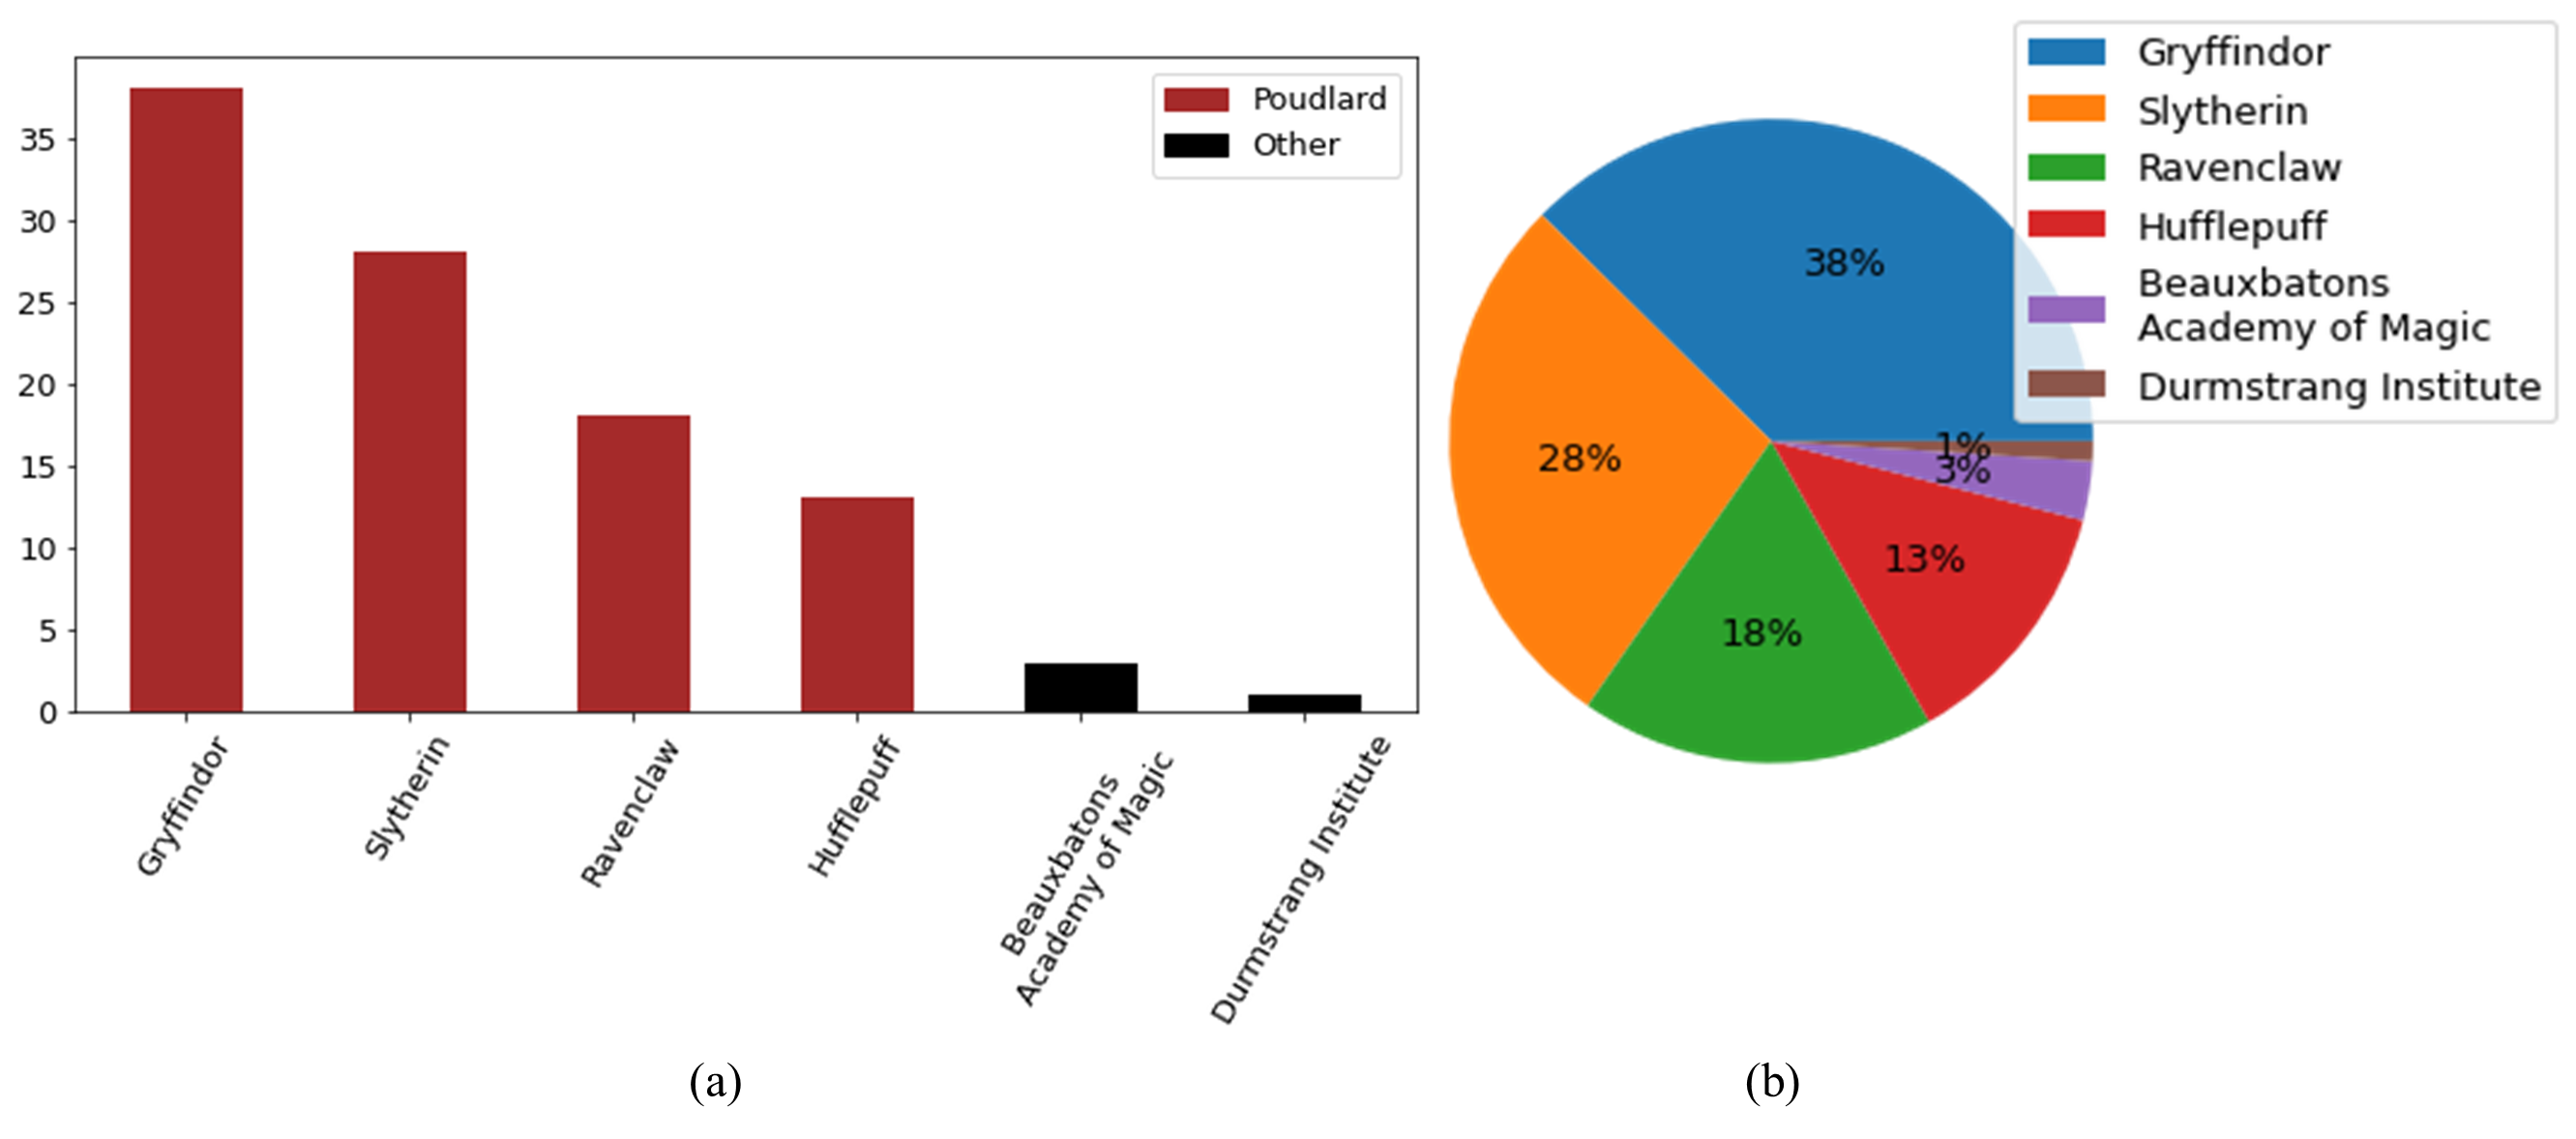
\includegraphics[width= 18 cm]{./figures/rep-houses.png}
    \caption{Regroupement des maisons et répartition des personnages par maison}
    \label{Regroupement}
\end{figure}
\FloatBarrier

La Figure \ref{Regroupement}.a représente la répartition des personnages selon les maisons.
Nous remarquons que 66\% des personnages appartiennent aux maisons Gryffindor et Slytherin.
En outre, nous constatons que le pourcentage des personnages des maisons "Beaubatons" et "Drumstrang" ne dépasse pas 4\%.
Selon la Figure \ref{Regroupement}.b, ces dernirrs appartiennent à des écoles différentes de Poudlard.\par

Nous étudions dans la suite le lien entre les caractéristiques des personnages (principalement le genre et le statut sanguin) et l'appartenance à une maison.\par

\begin{figure}[hbt!]
    \centering
    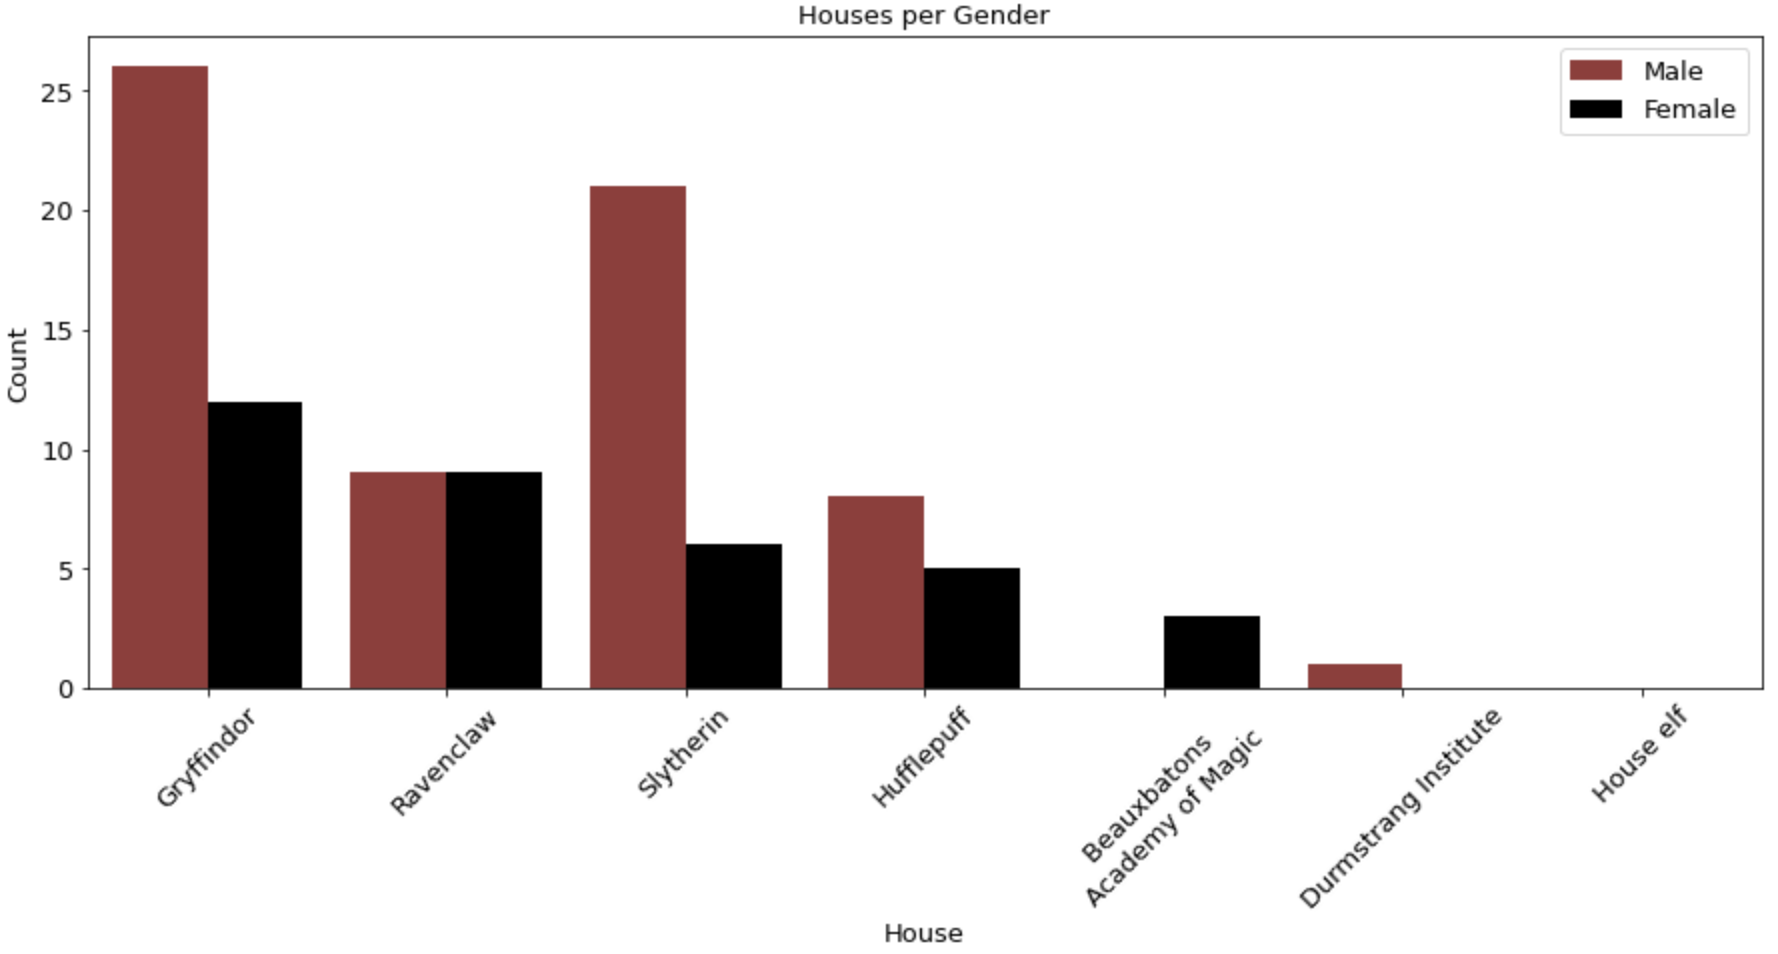
\includegraphics[width= 16 cm]{./figures/gender.png}
    \caption{Répartition des genres par maison}
    \label{Répartition}
\end{figure}
\FloatBarrier

La Figure \ref{Répartition} représente la répartition des personnages par genre dans chaque maison. Nous remarquons que les maisons de Poudlard contiennent des garçons et des filles, alors que les autres écoles sélectionnent selon le genre.\par

La Figure \ref{Sang} décrit les différents statuts sanguins présents dans chaque maison. Nous prennons le parti de prendre en considération cette variable car ,rappellons le, le statut de sang conditionne le statut du sorcier dans l'unvers d'Harry Potter.


\begin{figure}[hbt!]
    \centering
    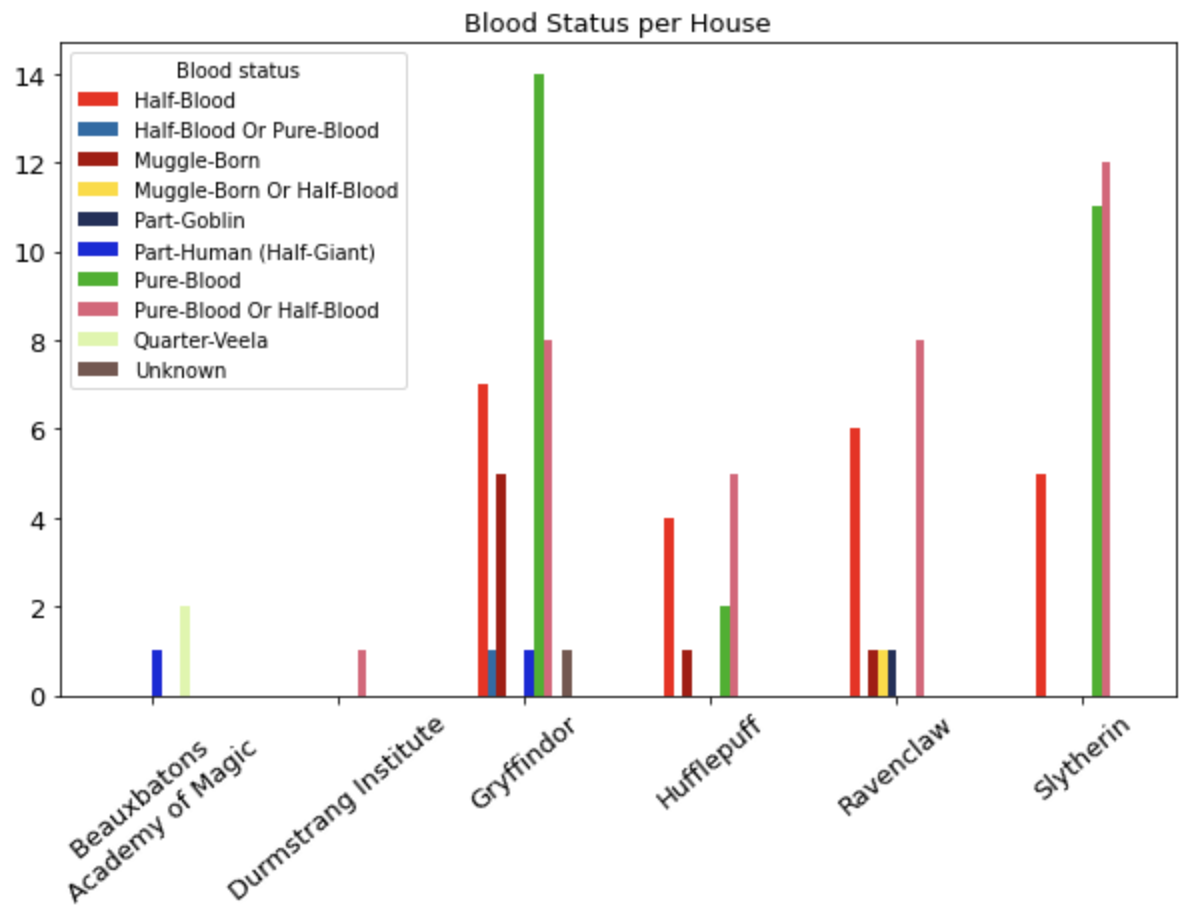
\includegraphics[width= 13cm, height= 8 cm]{./figures/blood_status.png}
    \caption{Répartition du statut de sang par maison}
    \label{Sang}
\end{figure}
\FloatBarrier

Nous remarquons que les sangs de type "Pure-Blood" et "Half-Blood" dominent toutes les maisons de l'école Poudlard. De plus, dans cette école, le type "Part-Human" caractérise une partie de personnages appartenant à la maison Gryffindor. La figure montre aussi que le type "Quarter-Veela" est absent de toutes les maisons sauf "Beauxbatons". Ces observations nous indiquent qu'il est légitime de considérer que le statut sanguin est une variable significative dans la classification des personnages.\par

Dans la suite, nous manipulons les données textuelles (les scripts) grâce à des méthodes de "text mining" pour savoir, dans la forme la plus courte possible, combien de fois parlent les personnages de ces trois films, ce qu'ils disent, quels mots ils utilisent souvent et bien plus encore.\par

Mais avant de "fouiller" dans le texte, nous commençons par regarder le nombre de phrases par personnage. La figure \ref{PersoPopuaire} représente les quinze personnages qui parlent le plus.

\begin{figure}[hbt!]
    \centering
    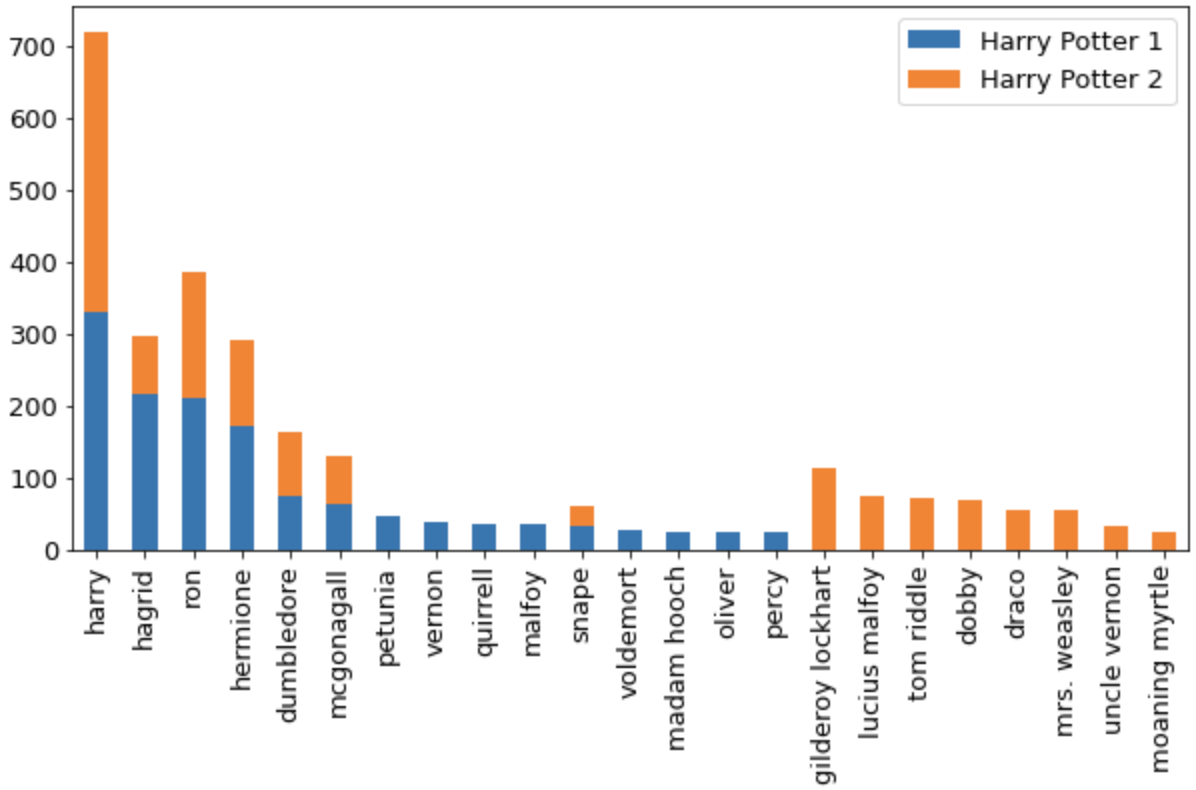
\includegraphics[width= 13cm, height= 8 cm]{./figures/most.png}
    \caption{Les personnages parlant le plus dans les deux premiers films}
    \label{PersoPopuaire}
\end{figure}
\FloatBarrier

On remarque que la première place est occupée par le personnage principal Harry Potter avec sept cent vingt phrases. En deuxième place, on trouve Ron, l'ami de Harry. De plus, au premier plan, nous trouvons de nombreux professeurs de Poudlard, les amis de Harry et le méchant de toute la saga - Lord Voldemort. Certains personnages n'apparaissent que dans une partie et parviennent quand même à figurer parmi les personnages avec le plus grand nombre de dialogues. Un tel personnage est Gilderoy Lockhart, qui a prononcé plus de cent discours dans la deuxième partie de la série de films.\par

Le "text mining" est l'art de transformer du texte libre en variables numériques, puis de les analyser avec des techniques statistiques. Afin d'appliquer cette analyse, nous avons effectué deux types de graphiques qui implémentent l'approche la plus courante du text mining : un wordcloud et des barplots de n-grammes (une séquence contiguë de n mots dans un texte. ).\par

La Figure \ref{Wordcloud} représente un wordcloud (nuage de mots-clés) avec tous les mots mentionnés au moins neuf fois dans le script des deux premiers films.

\begin{figure}[hbt!]
    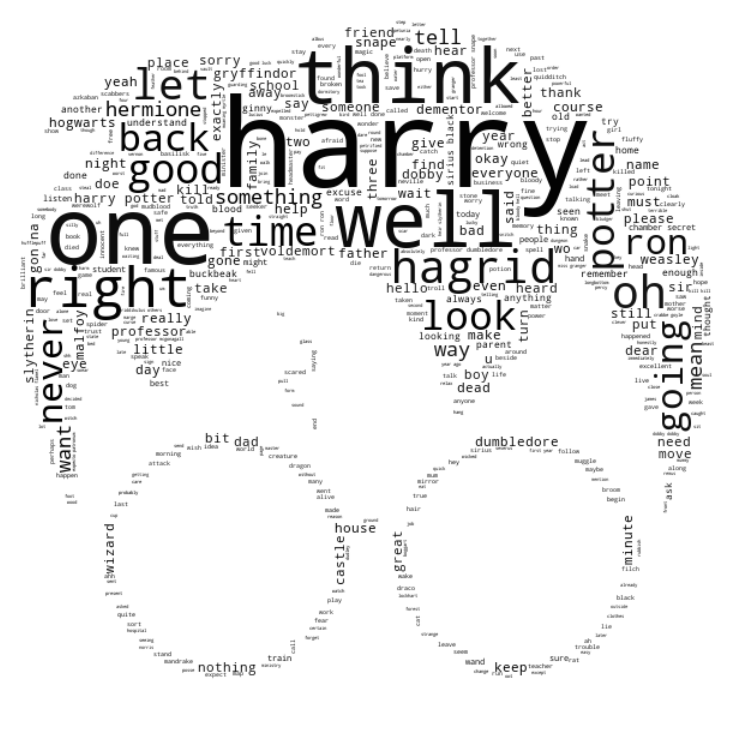
\includegraphics[width= 16cm]{./figures/wordcloud.png}
    \caption{Wordcloud des deux premiers films}
    \label{Wordcloud}
\end{figure}
\FloatBarrier

Les mots s'affichent dans des tailles et graisses de caractères d'autant plus visibles qu'ils sont utilisés ou populaires. Nous remarquons donc que le mot le plus populaire est "harry", qui représente le prénom du personnage principal. A part des mots du quotidien comme "one", "well", "think", d'autre prénoms de personnages apparaissent dont les plus populaires sont "hagrid", "ron" et "hermione" qui sont les amis proches de Harry.\par

Nous analysons dans la suite (Figure \ref{monograms}) les quinze monogrammes les plus populaires des deux premiers films.

\begin{figure}[hbt!]
    \centering
    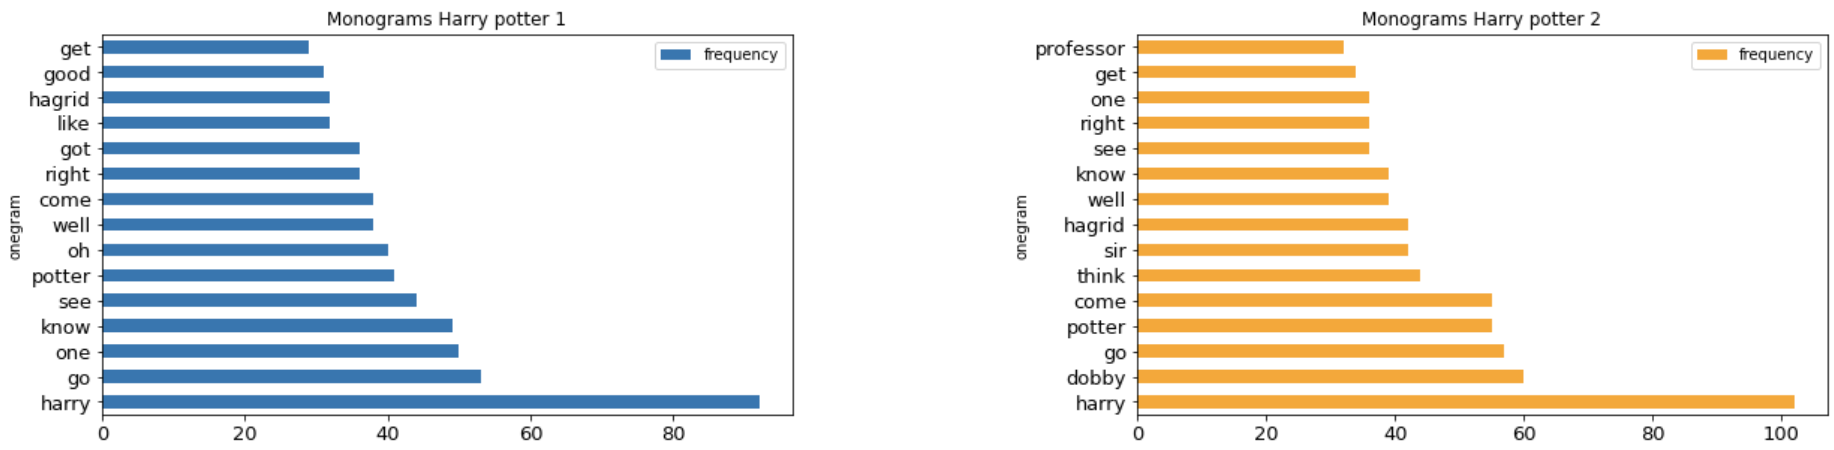
\includegraphics[width= 16cm, height= 7 cm]{./figures/monograms.png}
    \caption{Les quinze monogrammes les plus courants des deux premiers films}
    \label{monograms}
\end{figure}
\FloatBarrier

Dans cette analyse de monogrammes, nous remarquons que le mot "harry" est au sommet des mots prononcés. D'autres prénoms de personnages proches de Harry figurent dans la liste comme "hagrid" et "dobby". Cette analyse ronforce les résultats décrits précédemment.
On constate que tous ces mots varient trente et soixante à l'exception du prénom de personnage principal dépassant quatre-vingt-dix dans les deux films.\par

Une réflexion que l'on peut mener est que le personnage principal, ses amis et ceux qui intéragissent avec eux, influent fortement sur le script et par conséquent sur le choix des mots (en tant que variables explicatives) dans la matrice de design dans la partie suivante.

%------------------------------------------------------%
\subsection{Matrice de design}
%------------------------------------------------------%

Cette partie est consacrée à la construction de la matrice de design que nous noterons $X$ à laquelle seront appliquées les méthodes statistiques que nous développerons plus loin. Chacune de ses lignes correspond à un individu statistique, ici les personnages. Les colonnes de cette matrice contiennent les $p$ variables explicatives $(X_{1},...,X_{p})$  , que nous determinerons dans la suite, et la variable à expliquer $Y$ étant les maisons de Poudlard.\par

\subsubsection{Variable à expliquer}

Etant donné que notre but est de prédire l'appartenance d'un nouveau personnage à une maison, pour ne pas perdre de données qui nous serviront à alimenter les méthodes statistiques, nous choisissons d'inclure également les personnages n'appartenant à aucune des maisons de Poudlard sous la variable \textit{'Other'}. Ainsi nous obtenons cinq variables de "maison" ("Gryffindor", "Slytherin", "Ravenclaw", "Hufflepuff" et "Other") et pourrons inclure dans nos prédictions si un personnage n'apartient pas à une de maisons de Poudalard.\par

\newpage

\subsubsection{Variables explicatives}

En plus des variables de genre et de statut de sang vues précedemment nous considérons les variables suivantes issues des scripts : 

\begin{itemize}
    \renewcommand{\labelitemi}{$\bullet$}
    \item \textbf{Mots les plus communs :} En appliquant la fonction \textit{most\_common(10)} au script néttoyé, nous obtenons la liste des dix mots les plus prononcés et leur valeur correspondante :\\
    ('harry', 194), ('potter', 95), ('one', 86), ('well', 76), ('think', 75), ('hagrid', 74), ('right', 72), ('oh', 61), ('dobby', 60), ('would', 57).\\
    On remarque qu'en plus des noms de certains personnages, elle contient aussi des mots génériques ou encore une onomatopée, qui ne font partie de l'univers d'Harry Potter.\par
    Nous choisisons donc d'élargir la liste et de ne garder que dix mots liés à cet univers parmi les mots les plus dits :\\
    ('professor', 57), ('sir', 53), ('hogwarts', 38), ('slytherin', 38), ('school', 34), ('year', 33), ('gryffindor', 33), ('kill', 32), ('chamber', 32), ('wizard', 31).
    
    Les mots ainsi choisis sont placés dans les colonnes de la matrice $X$ et leur valeur correspond au nombre de fois que les personnages les ont prononcés ;

    \item \textbf{Fréquence des mots les plus communs :} Nous comptons le nombre de mots prononcés par chaque personnage et les ordonnons en fréquences.

\end{itemize}

Voici les premières lignes de la matrice de design obtenue pour les deux premiers films de la saga, à laquelle est ajoutée une colonne contenant les noms des personnages :

\begin{figure}[hbt!]
    \centering
    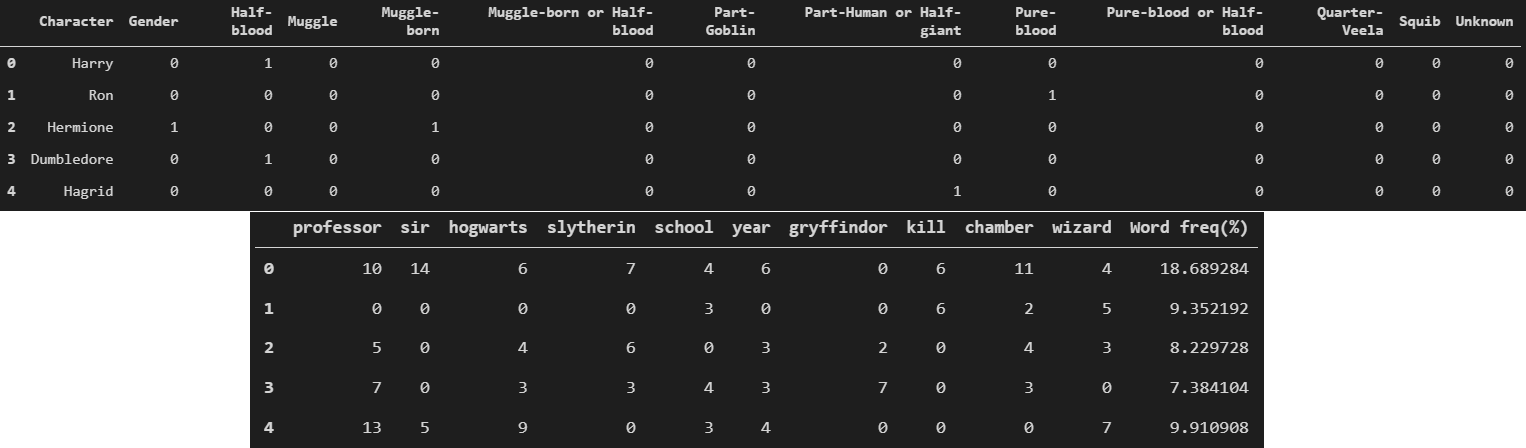
\includegraphics[width= 15.5 cm]{./figures/design.png}
    \caption{Matrice de design issue du script}
\end{figure}

\subsubsection{Variables additionnelles}

Nous pourrons par la suite, si les résultats statistiques le suggèrent, ajouter des caractérisques propres aux personnages, présentes dans les données "Characters.csv". En effet, les variables \textit{skills} et \textit{loyalty} pourront se révéler utiles quant à l'ajout d'information aux méthodes statistiques de classification.\par

\newpage

%------------------------------------------------------%
%------------------------------------------------------%
\section{Analyse statistique}
%------------------------------------------------------%
%------------------------------------------------------%

Soient dans la suite, $(n,p) \in \mathbf{N}^{2}$ la dimension de la matrice de design $X$ que nous avons construit dans la section précédente, $(x_{1}, x_{2}) \in \mathbb{R}^{p} \times \mathbb{R}^{p}$ deux observations issues de celle-ci et $y$ un élément de $Y \in \mathbb{R^n}$ le vecteur réponse.\par

La matrice de design correspond donc à l'ensemble des données étiquetées (i.e dont nous connaissons déjà la réponse cible). Ce sont nos données d'entrainement. Nous souhaitons connaître la relation entre $X$ et $Y$.\par

De manière plus formelle, l'objectif de la classification supervisée est de définir une fonction $h : x \mapsto y$ afin que pour une observation non connue $x$, $h(x)$ puisse prédire la sortie correpondante $y$.\par

Pour ce faire, la matrice de design nous permettra de construire un modèle statistique capable de classifier des personnages dans les maisons de Poudlard. Dans cette optique, nous entraînons plusieurs modèles de classification pour choisir le plus adapté à notre cas d'étude en se basant sur les métriques de performance.\par

%------------------------------------------------------%
\subsection{Validation croisée}
%------------------------------------------------------%

La validation croisée est, en apprentissage automatique, une méthode d’estimation de fiabilité d’un modèle fondé sur une technique d’échantillonnage.\cite{v} La prédiction se fait à partir d’un échantillon d’apprentissage pour ensuite être testée sur un échantillon test.\par

Cette méthode se généralise souvent en la validation croisée à $K$ groupes. Son fonctionnement est simple.
En effet, l’idée est de diviser les données en $K$ groupes de même taille et laisser le $k^{e}$ bloc de côté. Ensuite, on ajuste le modèle et on l’évalue sur le bloc laissé de côté. On répète l’opération en laissant de côté le bloc $k=1$, puis $k=2,\, \dots$ jusqu’à $k=K$. Enfin, on combine les résultats (sous forme de moyenne).\cite{K-cv}\par

Dans notre démarche statistique de l'implémentation des modèles de classification, nous serons donc amenés à optimiser les paramètres de ces derniers que nous allons tester et ce, par validation croisée. Il s'agit de chercher la précision optimale sur une grille de paramètres.\par

Nous utilisons la bibliothéque \textit{sk\_learn} de python pour implémenter nos deux modèles. Nous ferons appel par la suite à la classe \textbf{GridSearchCV} du module \textit{model\_selection} afin de déterminer ces paramètres optimaux.

%------------------------------------------------------%
\subsection{Méthode des k plus proches voisins}
%------------------------------------------------------%

L’algorithme des k plus proches voisins (K-nearest neighbors en anglais, abrégé k-NN) est un algorithme de Machine Learning qui appartient à la classe des algorithmes d’apprentissage supervisé.
Simple et facile à mettre en œuvre car son algorithme repose uniquement sur le choix de la métrique de classification, notée $k$. Il est de plus “non paramétrique” (seul $k$ doit être fixé) et se base uniquement sur les données d’entraînement.{\cite{k-nn}}
Cet algorithme peut être utilisé pour résoudre les problèmes de classification et de régression.{\cite{3}}\par

\subsubsection{Principe :}

Son principe est simple. Afin de déterminer la classe d'un individu n'appartenant pas au jeu de données, l'algorithme calcule la distance de celui-ci à tous les autres, collecte les classes des $k$ individus les plus proches et effectue un vote majoritaire dont la résultante sera la classe prédite pour le nouvel individu.\par

Cette méthode est souvent qualifiée de \textit{Lazy learner} provenant du fait qu'elle n'aie pas besoin de phase d'apprentissage.
En effet k-NN stocke l'ensemble des données et se base dessus afin d'effectuer une prédiction.\par

\subsubsection{Algorithme :}

Récapitulons maintenant les étapes du k-NN :

    \begin{itemize}
        \item Entrées :
            \begin{itemize}
                \item Un jeu de données ;
                \item Une distance d ;
                \item Un nouvel individu $x \in \mathbf{R}^{p}$ à classifier ;
                \item Un nombre entier $k$.
            \end{itemize}
            
        \item Traitement :
            \begin{enumerate}
                \item Calcul des distances entre $x$ et tous les points du jeu de données ;
                \item Détermination des $k$ plus proches "voisins" ;
                \item Collection des classes de ces $k$ points ;
                \item Attribution de la classe la plus présente à $x$.
            \end{enumerate}
        
        \item Sortie : Classe prédite de $x$.
    \end{itemize}

Voici un exemple graphique pour illustrer cette méthode :

\begin{figure}[hbt!]
    \centering
    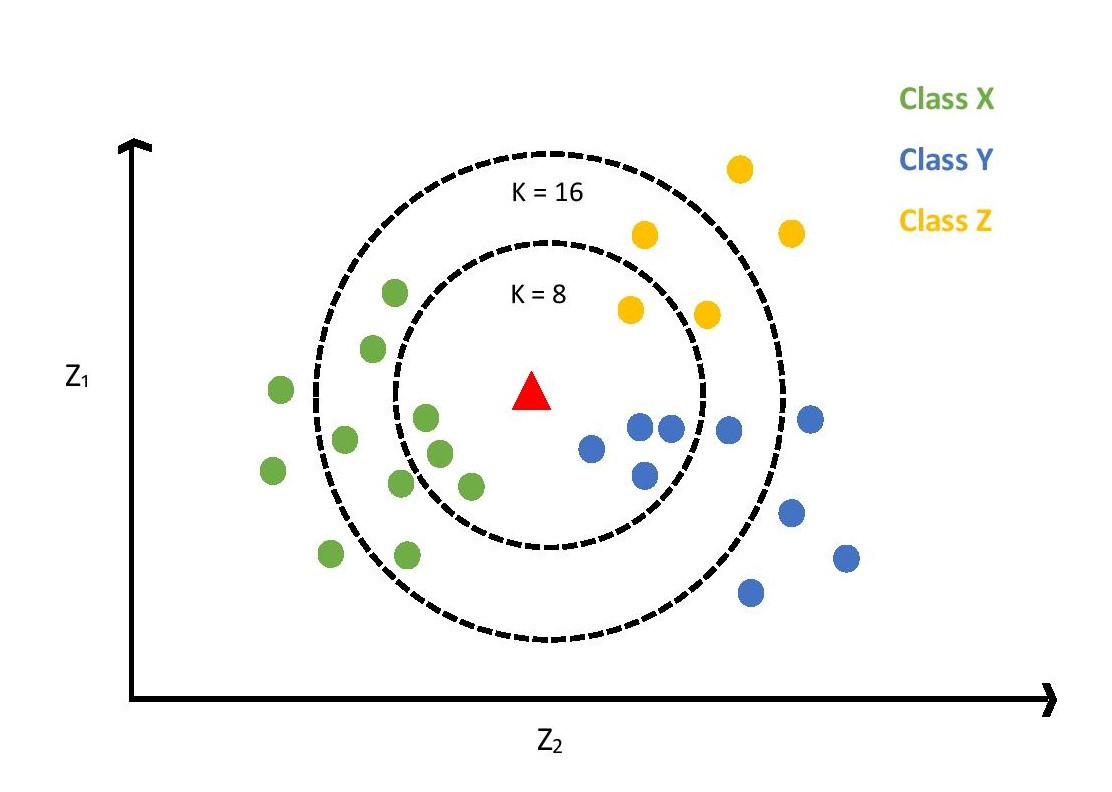
\includegraphics[width = 15 cm, height = 9 cm]{./figures/knn_example.jpeg}
    \caption{Exemple d'un algorithme k-NN (source: \cite{5}, auteur: Tharuka Sewwandi).}
    \label{12}
\end{figure}
\FloatBarrier

\subsubsection{Paramètres et implémentation :}

Le but de cette partie est de déterminer, grâce aux données des deux premiers films présentes dans la matrice de design, les hyperparamètres du modèle k-NN en vue de l'appliquer au toisième film.\par

\begin{itemize}
    \item \textbf{Le nombre de voisins $k$ ("n\_neighbors") :}
    Sur la figure \ref{12} on remarque que selon la valeur de $k$, la classe du nouvel individu change. En effet, sur cet exemple si $k=8$ la classe attribuée est $Y$, alors que si $k=16$, le nouveau point appartient à la classe $X$. Ceci illustre bien l'importance du choix du paramètre $k$ ;\par
    
    \item \textbf{La fonction de distance ("metric") :}
    Comme dit plus haut, le k-NN nécessite une fonction de calcul entre deux individus (observations) afin d'évaluer la notion de "similarité". Plus la distance est petite, plus les individus sont similaires.
    On note à ce titre, plusieurs distances pouvant être utilisées selon le type de données. Par défaut, la distance euclidienne $d_{e}(x_{1}, x_{2})=\sqrt{\sum_{j=1}^{p}\left(x_{1_j}-x_{2_j}\right)^{2}}$ est implémentée ;

    \item \textbf{Le poids des individus ("weights") :}
    L'algorithme k-NN propose d'affecter ou pas des poids aux individus en fonction de leur distance au nouveau point.
        \begin{itemize}
        \renewcommand{\labelitemii}{-}
            \item "uniform" : l'ensemble des individus du jeu de données ont un même poids ;
            
            \item "distance" : plus un individu est proche/similaire (au sens de la métrique) du nouveau point, plus son poids est grand.
        \end{itemize}
\end{itemize}

Nous déterminons à présent ces paramètres en essayant toutes les combinaisons possibles pour en comparer les scores.
Nous faisons donc appel la fonction GridSearchCV. 

\begin{figure}[hbt!]
    \centering
    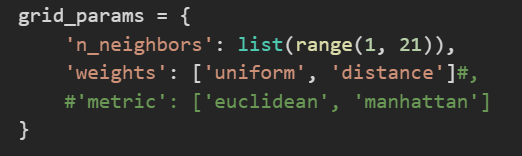
\includegraphics[width = 9 cm]{./figures/k.PNG}
    \caption{Hyperparamètres à optimiser (k-NN)}
    \label{param_opti-k-nn}
\end{figure}
\FloatBarrier

\textit{Remarques : }\par
\begin{itemize}

    \item En fixant \texit{n\_jobs} à $-1$, nous demandons à l'ordinateur d'utiliser tous ses processeurs pour effectuer le modèle sauf un ;{\cite{med}}

    \item Autre élément important à mentionner, GridSearchCV exécute plusieurs modèles. Dans l'implémentaion ci-dessus nous avons : vingt possibilités pour le paramètre \texit{n\_neighbors}, deux possibilités pour le paramètre \texit{weights}. Si par exemple nous effectuons onze validations croisées, cela porte le total à $2*11*20 = 440$ ;

    \item Le temps d'exectuion croît en même temps que la dimension de $X$ car la fonction mesure les distances entre $x$ et tous les points du jeu de données. C'est donc une méthode qui peut s'avérer coûteuse.
\end{itemize}

\newpage

Voici la combinaison ayant obtenu la meilleure précision :

\begin{figure}[hbt!]
    \centering
    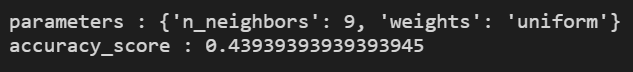
\includegraphics[width = 14 cm]{./figures/kNN_grid1.png}
    \caption{Hyperparamètres optimaux du k-NN.}
    \label{param_knn1}
\end{figure}
\FloatBarrier
Notons que l'\textit{accuracy\_score} correspond au taux de bon classement.

En plus de rechercher les meilleurs paramètres et la précision associée, la fonction GridSearchCV effectue une validation croisée afin d'évaluer l'algorithme k-NN avec ces derniers.
Notons que cette fonction automatise aussi la stratification (il faut affecter un nombre de plis au paramètre "\textit{cv}") des données d'entraînement et de test lors de la validation croisée.
Ainsi nous évitons que le modèle fasse de \textit{l'over-fitting}, à savoir le fait qu'il ne colle trop à la structure des données. En effet dans notre cas, les classes sont inégalement réparties :

    \begin{itemize}
        \item "Gryffindors" : 34
        \item "Slytherins" : 26
        \item "Ravenclaws" : 17
        \item "Hufflepuffs" : 13
        \item "Others" : 42,
    \end{itemize}

\subsubsection{Prédictions :}

Après avoir fixé les hyperparamètres de notre modèle, nous l'appliquons enfin au troisième film.\par
Voici la liste des nouveaux personnages apparaissant dans \texit{Harry Potter 3} dont nous cherchons à prédire la maison :
    \begin{align*}
        Sirius, Lupin, Pettigrew, Parvati Patil, Trelawney, Goyle, Pansy Parkinson et Aunt Marge.
    \end{align*}

Nous obtenons ainsi le vecteur des prédictions suivant (Figure \ref{res_knn1}) et une précision de 25\%. 
\begin{figure}[hbt!]
    \centering
    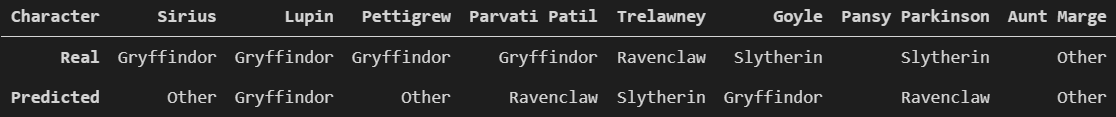
\includegraphics[width = 14 cm]{./figures/output_knn1.png}
    \caption{Comparaison des vraies classes à celles prédites}
    \label{res_knn1}
\end{figure}
\FloatBarrier

Néanmoins, nous nous demandons si ajouter d'autres variables explicatives telles que les compétences et la loyauté peut améliorer cette prédiction.\par

Nous piochons donc ces informations dans le fichier csv "\textit{Characters}" et les ajoutons à la matrice de design.
Nous appliquons alors une nouvelle fois la recherche d'hyperparamètres avec cette nouvelle matrice de design ;

\begin{figure}[hbt!]
    \centering
    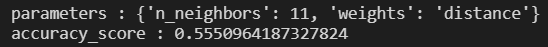
\includegraphics[width = 12 cm]{./figures/kNN_grid2.png}
    \caption{Hyperparamètres optimaux du second modèle k-NN}
    \label{param_knn2}
\end{figure}
\FloatBarrier

et obtenons une précision de prédiction de 50\%, soit deux fois plus que pour le précedent modèle.

\begin{figure}[hbt!]
    \centering
    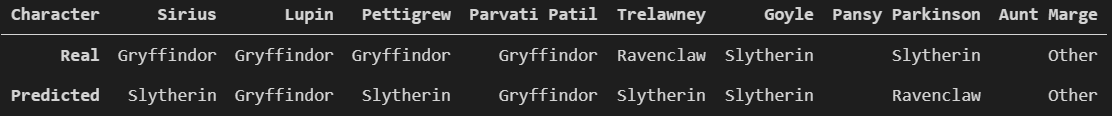
\includegraphics[width = 14 cm]{./figures/output_knn2.png}
    \caption{Comparaison des vraies classes à celles prédites par le second modèle}
    \label{res_knn2}
\end{figure}

%------------------------------------------------------%
\subsection{Forêts Aléatoires (Random Forests)}
%------------------------------------------------------%

\subsubsection{Arbres de décision}

Le modèle \textbf{"Arbre de décision"} représente une pierre angulaire des forêts aléatoires. Ce modèle structure les données sous la forme d'un arbre. Il est construit de deux types d'éléments: les \textbf{nœuds} et les \textbf{branches}. Un \textbf{nœud} correspond à un test sur un attribut ou \textit{feature} (variable explicative). À chaque \textbf{nœud}, l'attribut est donc évalué pour prendre une décision de séparation, comme le montre la Figure \ref{tree} ci-après. Les branches sont les résultats de ces tests et les feuilles de l'arbre correspondent aux classes. L'objectif est de réduire l'impureté totale des deux nœuds fils par rapport au nœud père à chaque étape de séparation.

\begin{figure}[hbt!]
    \centering
    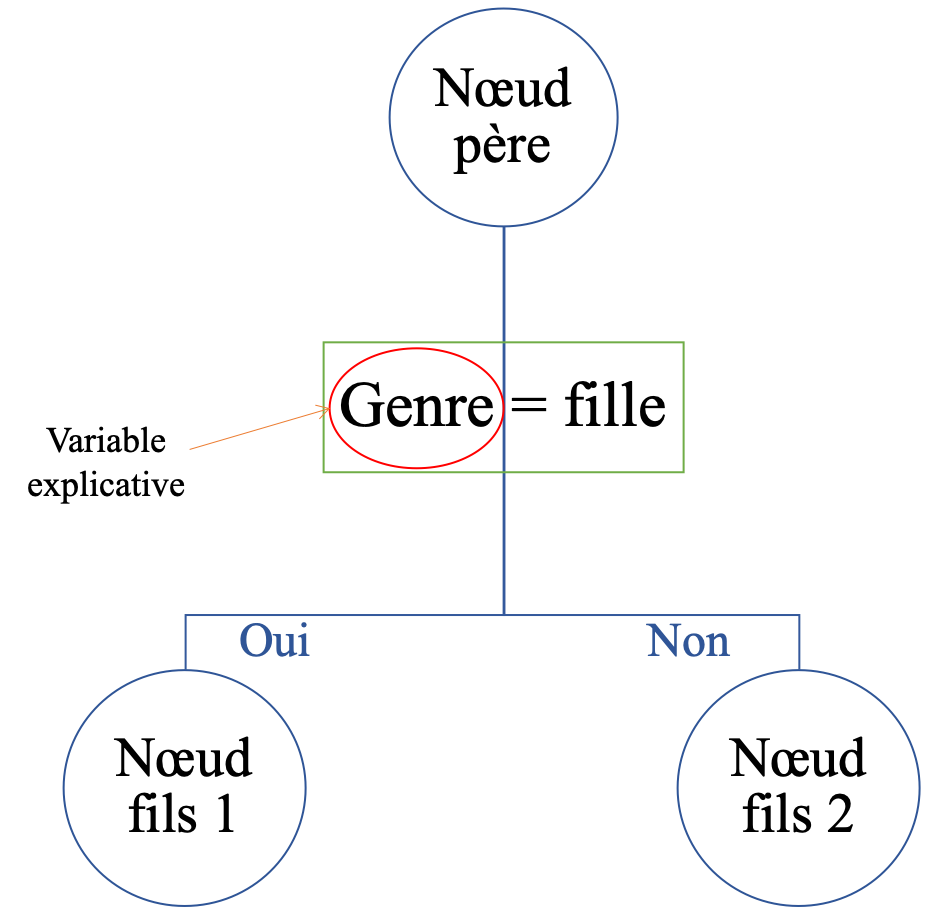
\includegraphics[width = 7 cm]{./figures/tree.png}
    \caption{Exemple simple d'arbre de décision}
    \label{tree}
\end{figure}
\FloatBarrier

De ce fait, la classification d'un nouvel individu se fait en testant les attributs de celui-ci les uns à la suite des autres.\par

Malgré les avantages fournis par le modèle d'arbre de décision tels que la simplicité, la transparence et l’interprétabilité des prédictions, ce modèle envisage des difficultés de stabilité. A titre d'exemple, la génération d'un nouvel arbre à chaque petite modification des données d’entraînement et de sur-apprentissage dans le cas de la création d'un arbre complexe pour des données simples \cite{hands}.\par

Afin de surmonter ces difficultés, le modèle de \textbf{forêt aléatoire} permet d'avoir une prédiction plus précise et plus stable grâce à l’agrégation des prédictions provenant d'un ensemble d'arbres de décision.\par

\subsubsection{Principe :}

Le modèle Random Forest \cite{598994}\cite{breiman2001random}, abrégé RF, se base premièrement sur la méthode du \textbf{Bagging} (pour \textbf{Bootsrap Aggregating}). Cette méthode consiste à échantillonner de manière aléatoire des sous-ensembles de données d'entraînement, appelé bootstrap.
Deuxièmement, une méthode de \textbf{randomisation} est appliquée afin de selectionner de manière aléatoire un sous-ensemble de variables explicatives parmi les données échantillonnées. Ces données sont ensuite utilisées pour entraîner un nombre défini d'arbres de décision.
Une fois que tous ces prédicteurs sont formés, l'ensemble peut faire une prédiction pour une nouvelle instance en utilisant le \textbf{vote majoritaire} comme méthode d’agrégation de tous les prédicteurs. Ce processus est décrit dans la Figure \ref{RF}.\par

\begin{figure}[hbt!]
    \centering
    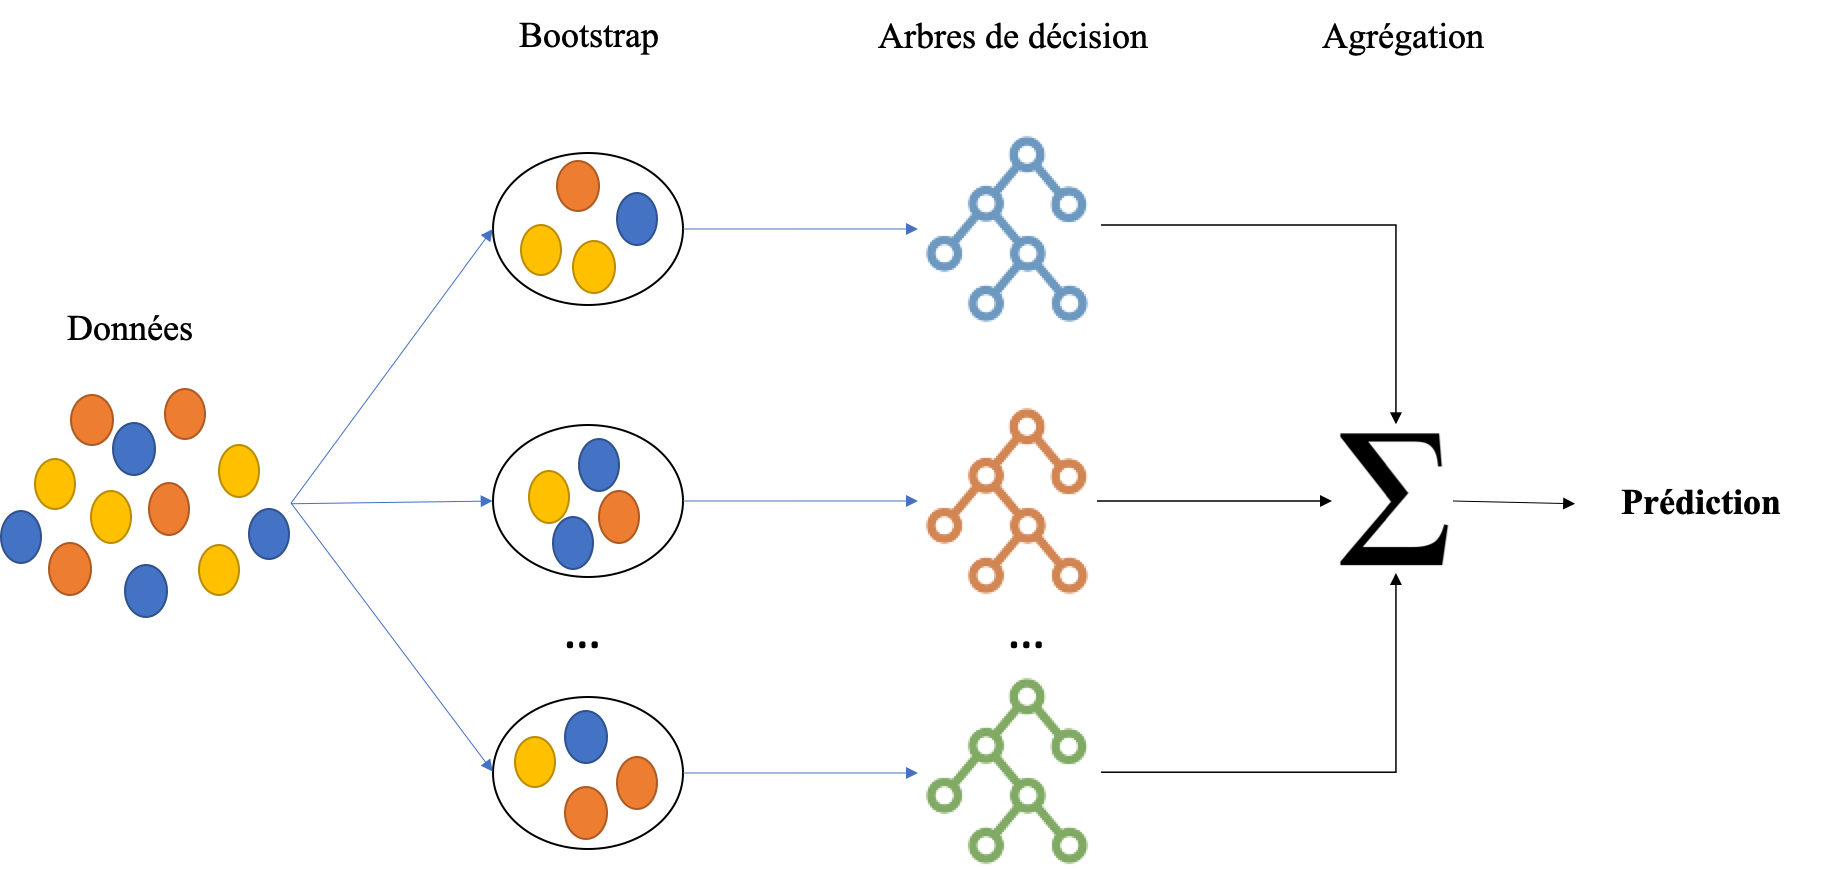
\includegraphics[width = 15 cm]{./figures/RF.png}
    \caption{Processus Random Forest}
    \label{RF}
\end{figure}
\FloatBarrier

\newpage

\subsubsection{Algorithme :}

Récapitulons maintenant les étapes du RF :

    \begin{itemize}
        \item Entrées :
            \begin{itemize}
                \item Un jeu de données ;
                \item Un nombre entier $N$ d’arbres de décision.
            \end{itemize}
            
        \item Entraînement :
            \begin{enumerate}
                \item Créer $N$ échantillons du jeu de données ;
                \item Sélectionner aléatoirement $m$ variables explicatives avec $m < M$ où $M$ est le nombre total des variables explicatives ;
                \item Créer $N$ arbres de décision, et entraîner chacun d'eux sur un échantillon différent ;
                \item Effectuer une prédiction finale en agrégeant les prédictions des arbres.
            \end{enumerate}
        
        \item Sortie : classe prédite de $x$.
    \end{itemize}

\subsubsection{Paramètres et implémentation :}

Dans le cadre de notre étude, nous utilisons l'objet RandomForestClassifier de la bibliothèque scikit-learn \cite{4}. Ses paramètres les plus importants sont :

\begin{itemize}
    \item \textbf{max\_features :} nombre de features/attributs à chaque découpage d'arbre. Il s'agit du nombre de variables tirées aléatoirement pour la recherche de la division optimale d'un noeud \cite{dobby} ;
    \item \textbf{n\_estimators :} nombre d'arbres. C'est un paramètre de type entier. Il est égal à 100 par défaut ;
    \item \textbf{max\_depth :} nombre maximal de niveau d'arbre de décision ;
    \item \textbf{criterion :} fonction permettant de mesurer la qualité du découpage d'arbre ;
    \item \textbf{class\_weight :} poids associés aux classes.
\end{itemize}

Nous faisons appel à la classe \textbf{GridSearchCV}, qui on rappelle, nous permet d'automatiser la recherche d'un optimum parmi les hyperparamètres décrits dans la Figure \ref{paramtunRF} en effectuant une validation croisée de dix plis dans ce cas.\par

\begin{figure}[hbt!]
    \centering
    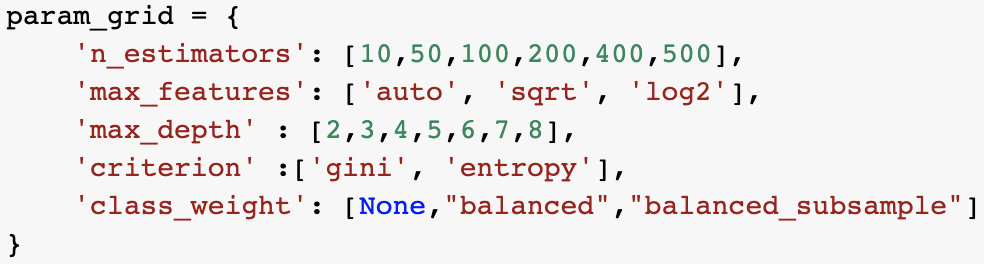
\includegraphics[width= 13 cm]{figures/paramtunRF.png}
    \caption{Hyperparamètres à optimiser (RF)}
    \label{paramtunRF}
\end{figure}
\FloatBarrier

Nous appliquons GridSearchCV sur les variables extraites purement des données textuelles en les répartissant en 80\% pour l’entraînement et 20\% pour le test. Nous obtenons les paramètres suivants :

\begin{figure}[hbt!]
    \centering
    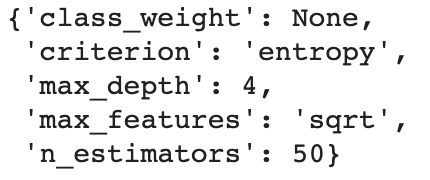
\includegraphics[width = 7 cm]{./figures/outputCVRF.png}
    \caption{Hyperparamètres optimaux}
    \label{CV1}
\end{figure}
\FloatBarrier

Nous entraînons notre modèle en se basant sur ces derniers résultats. Nous obtenons une précision sur les données du test d'environ 27\%.

La matrice de confusion est un outil résumant les résultats de prédictions. Les prédictions correctes et incorrectes sont mises en lumière et réparties par classe. Les prédictions sont ainsi comparés avec les valeurs réelles.

\begin{figure}[hbt!]
    \centering
    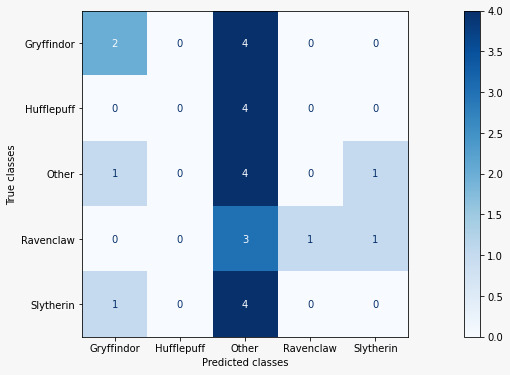
\includegraphics[width= 11 cm]{figures/matriceconfRF.jpeg}
    \caption{Matrice de confusion RF}
    \label{confRF}
\end{figure}
\FloatBarrier

La diagonale représente les bonnes prédictions. Nous remarquons donc que le modèle a bien prédit la classe "Other". En revanche, il n'arrive pas à bien distinguer les autres classes ; 57\% des personnages qui appartiennent à d'autres classes sont prédits comme appartenant à "Other".\par

Afin d’améliorer notre modèle, nous avons ajouté aux données textuelles des variables caractéristiques qui décrivent chaque personnage. Nous ré-entraînons ce nouveau modèle de la même façon que le premier et obtenons les résultats suivants :

\begin{figure}[hbt!]
    \centering
    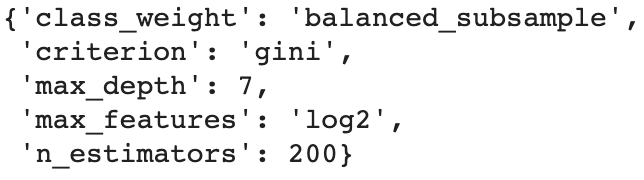
\includegraphics[width= 9 cm]{figures/outputCVRF2.png}
    \caption{Hyperparamètres optimaux}
    \label{CV2}
\end{figure}
\FloatBarrier

Après l’entraînement d'un nouveau modèle utilisant les paramètres de la Figure \ref{CV2}, nous remarquons que la précision de prédiction est passée de 27\% à environ 61,5\%, ce qui signifie que les variables liées aux personnages ont pu aider le modèle à mieux distinguer les différentes classes.
La matrice de confusion (Figure \ref{confRF2}) illustre ces nouvelles performances.

\begin{figure}[hbt!]
    \centering
    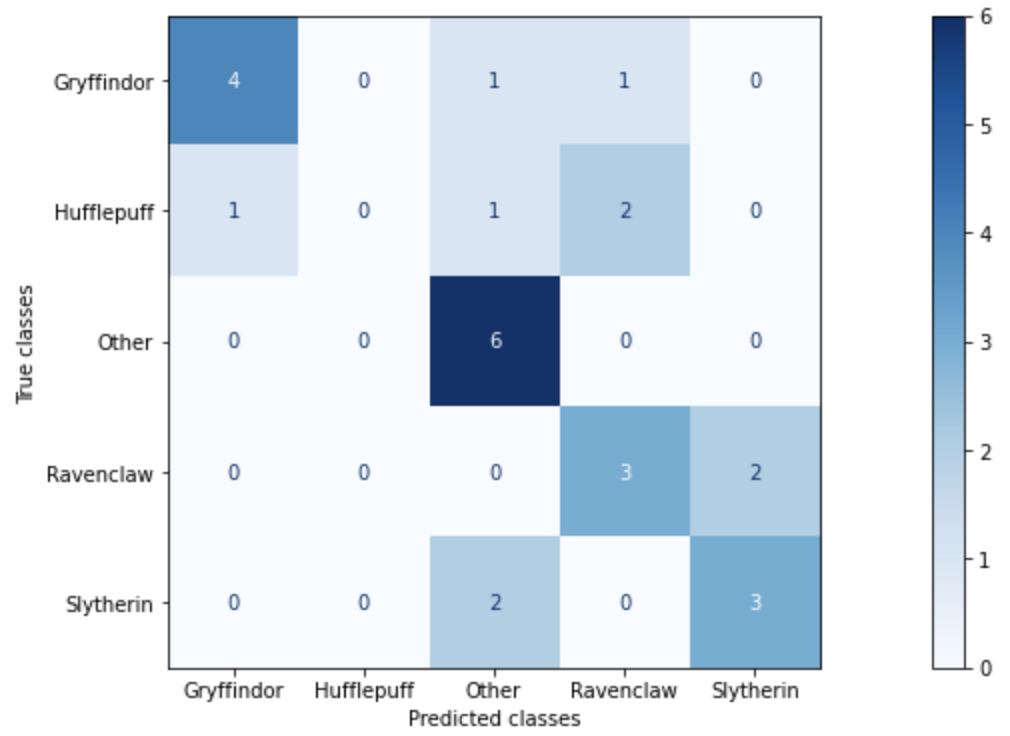
\includegraphics[width = 11 cm]{figures/matriceconfRF2.png}
    \caption{Matrice de confusion du second RF}
    \label{confRF2}
\end{figure}
\FloatBarrier

Cependant, le modèle n'a pas pu encore distinguer la maison "Hufflepuff", ce qui signifie qu'il a probablement besoin d'autres variables explicatives.\par

En se basant sur la precision des deux modèles Random Forest, nous choisissons le deuxième pour tester sa capacité à classifier les nouveaux personnages du troisième film. Nous obtenons finalement une précision de 25\%.

\begin{figure}[hbt!]
    \centering
    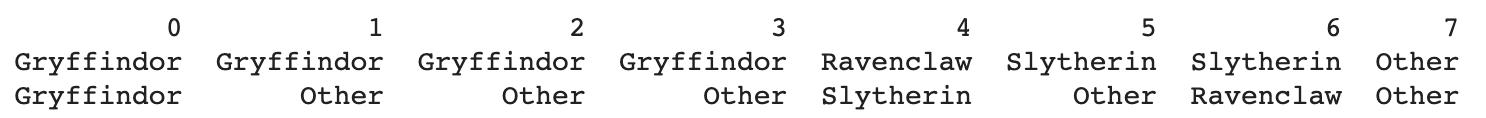
\includegraphics[width = 16 cm]{figures/finalresults.png}
    \caption{Résultat des prédictions (deuxième ligne) sur le troisième film}
    \label{finalresult}
\end{figure}
\FloatBarrier

\subsection{Conclusion}

La meilleure précison obtenue sur les prédictions des maisons des nouveaux personnages du troisième film est de 50\% avec le modèle k-NN. C'est un premier résultat encourageant car supérieur à un classifieur aléartoire, néanmoins, il tend à être amélioré.
En effet, une analyse des données de test (troisième film) révèle que le discours des personnages sélectionnés n’est pas suffisamment adapté à la matrice de design ; les mots utilisés comme variables explicatives sont moins prononcés, voire inemployés dans le troisième film.

\newpage

%------------------------------------%
%------------------------------------%
\section{Conclusion générale}
%------------------------------------%
%------------------------------------%

Ce rapport propose une analyse statistique de la saga Harry Potter dans le but d'implémenter un modèle de classification supervisée de personnages selon les maisons de Poudlard. Deux axes ont formé l'épine dorsale de ce travail :

\begin{itemize}
    \renewcommand{\labelitemi}{-}
    \item L'analyse de données où nous avons effectué une étude sur les scripts et les caractéristiques des personnages afin de définir des variables explicatives permettant de les classifier ;
    \item L'implémentaion des modèles statistiques k-NN et forêt aléatoire pour classifier les personnages.
\end{itemize}

A partir des résultats de ces deux axes, nous concluons que les performances des modèles implémentés peuvent être améliorées grâce à des manipulations sur les données textuelles comme la collecte de nouvelles données, la correction des données ou encore l'extraction de nouvelles variables explicatives. Dans ce contexte, deux perspectives se présentent :

\begin{itemize}
    \renewcommand{\labelitemi}{-}
    \item Utilisation d'une analyse sémantique des mots c-à-d se concentrer sur la signification contextuelle des mots au lieu d'étudier son existence dans le texte ; par exemple le mot "tuer" peut être prononcé comme "assassiner" ou "éliminer" ;
    
    \item Une extraction des connaissances à partir des scripts au lieu d'utiliser des mots prononcés par les personnages. Pour cela, nous proposons une analyse préliminaire d'une nouvelle approche basée sur l'analyse sentimentale. L'annexe \ref{A1} fournit une étude préliminaire prometteuse de cette approche.
\end{itemize}

\newpage

\appendix

%------------------------------------------------------%
%------------------------------------------------------%
\section{Annexe}
%------------------------------------------------------%
%------------------------------------------------------%

%-----------------------------------------------------------%
\subsection{Annexe 1 : modèle basé sur l'analyse sentimentale}\label{A1}
%-----------------------------------------------------------%

\subsubsection{Etude des n-grammes :}

\begin{figure}[hbt!]
    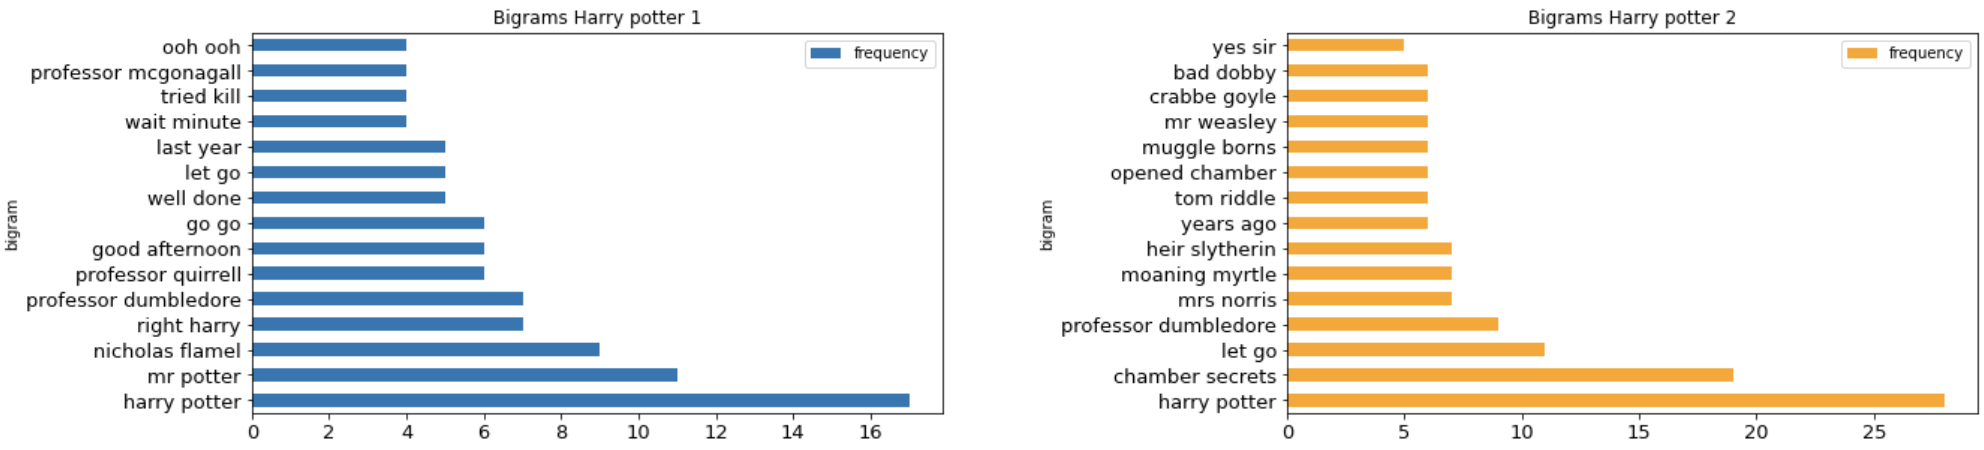
\includegraphics[width= 16cm, height= 7 cm]{./figures/bigrams.png}
    \caption{Les quinze bigrammes les plus fréquents des deux premiers films}
    \label{bigrams}
\end{figure}
\FloatBarrier

Le bigramme le plus employé est "harry potter", qui est apparu dans les deux premiers opus de la saga quarente-sept fois au total. Parmi les personnages, figurent également "nicholas flamel", "tom riddle", "professor dumbledore", "mrs morris", etc. La place suivante est occupée par des expressions courantes du telles que "good afternoon", "well done", ou encore "yes sir". Un bigramme dans le deuxième chapitre semble intéressant et unique : "heir slytherin".\par

La Figure \ref{trigrams} représente les quinze trigrammes les plus prononcés dans les films 1 et 2.

\begin{figure}[hbt!]
    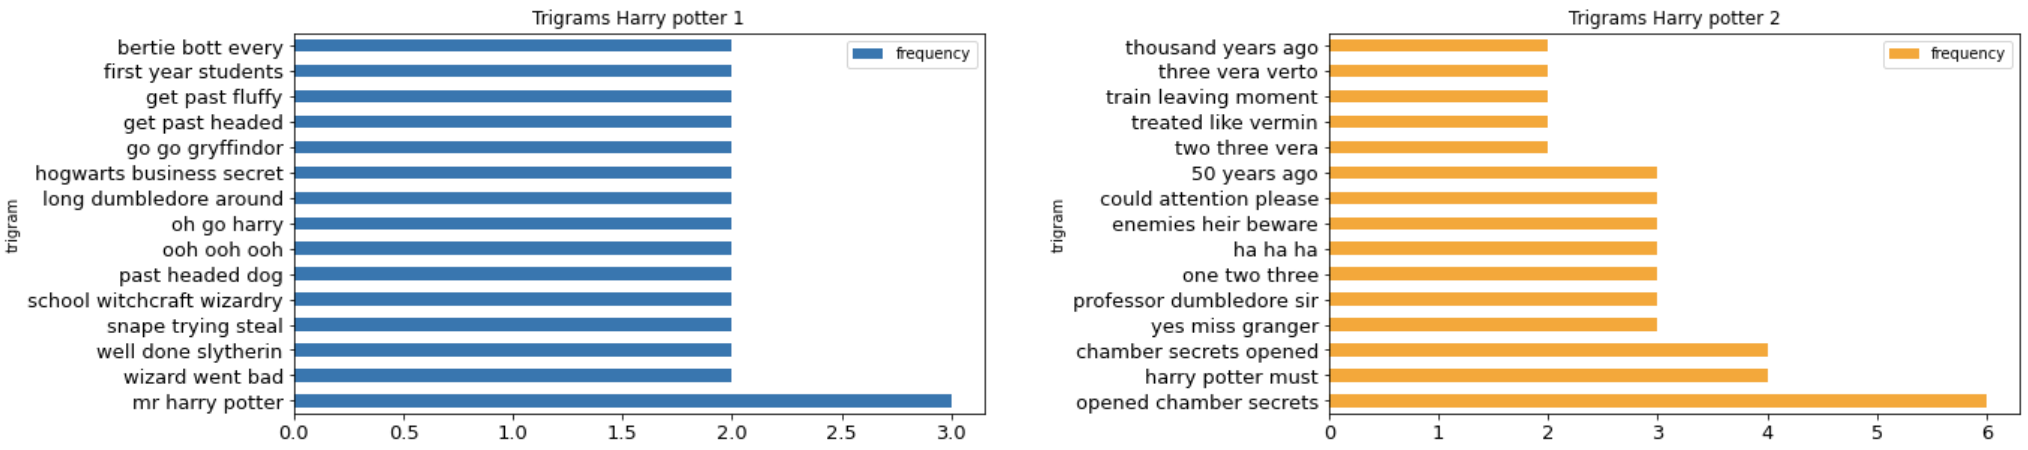
\includegraphics[width= 16cm, height= 7 cm]{./figures/trigrams.png}
    \caption{Les quinze trigrammes les plus fréquents des deux premiers films}
    \label{trigrams}
\end{figure}
\FloatBarrier

Nous remarquons que les trigrammes ont des fréquences plus petites car une séquence de trois mots dans le même ordre est beaucoup moins courante qu'une séquence de deux mots.
Une partie du titre du deuxième film "opened chamber secrets" s'est avérée être le trigramme le plus prononcé dans ce chapitre. Alors que pour le premier film, le trigramme le plus récurrent "mr harry potter" fait encore référence au personnage principal. Dans ces trigrammes , mis à part les phrases bien connues du discours quotidien, les éléments intéressants sont "hogwart business secret" et "school witchcraft wizardry", que nous ne trouverons certainement pas ailleurs.\par

L'analyse émotionnelle représente une des applications les plus utilisées dans le NLP. Dans cette optique, nous exploitons le traitement de texte effectué précédemment pour étudier le degré d'affect émotionnel dans le discours des personnages.\par

Dans un premier temps, nous étudions la polarité des n-grammes en utilisant le module VADER (Valence Aware Dictionary and sEntiment Reasoner) implémenté au niveau de la bibliothèque \textit{NLTK}.

\begin{figure}[hbt!]
    \centering
    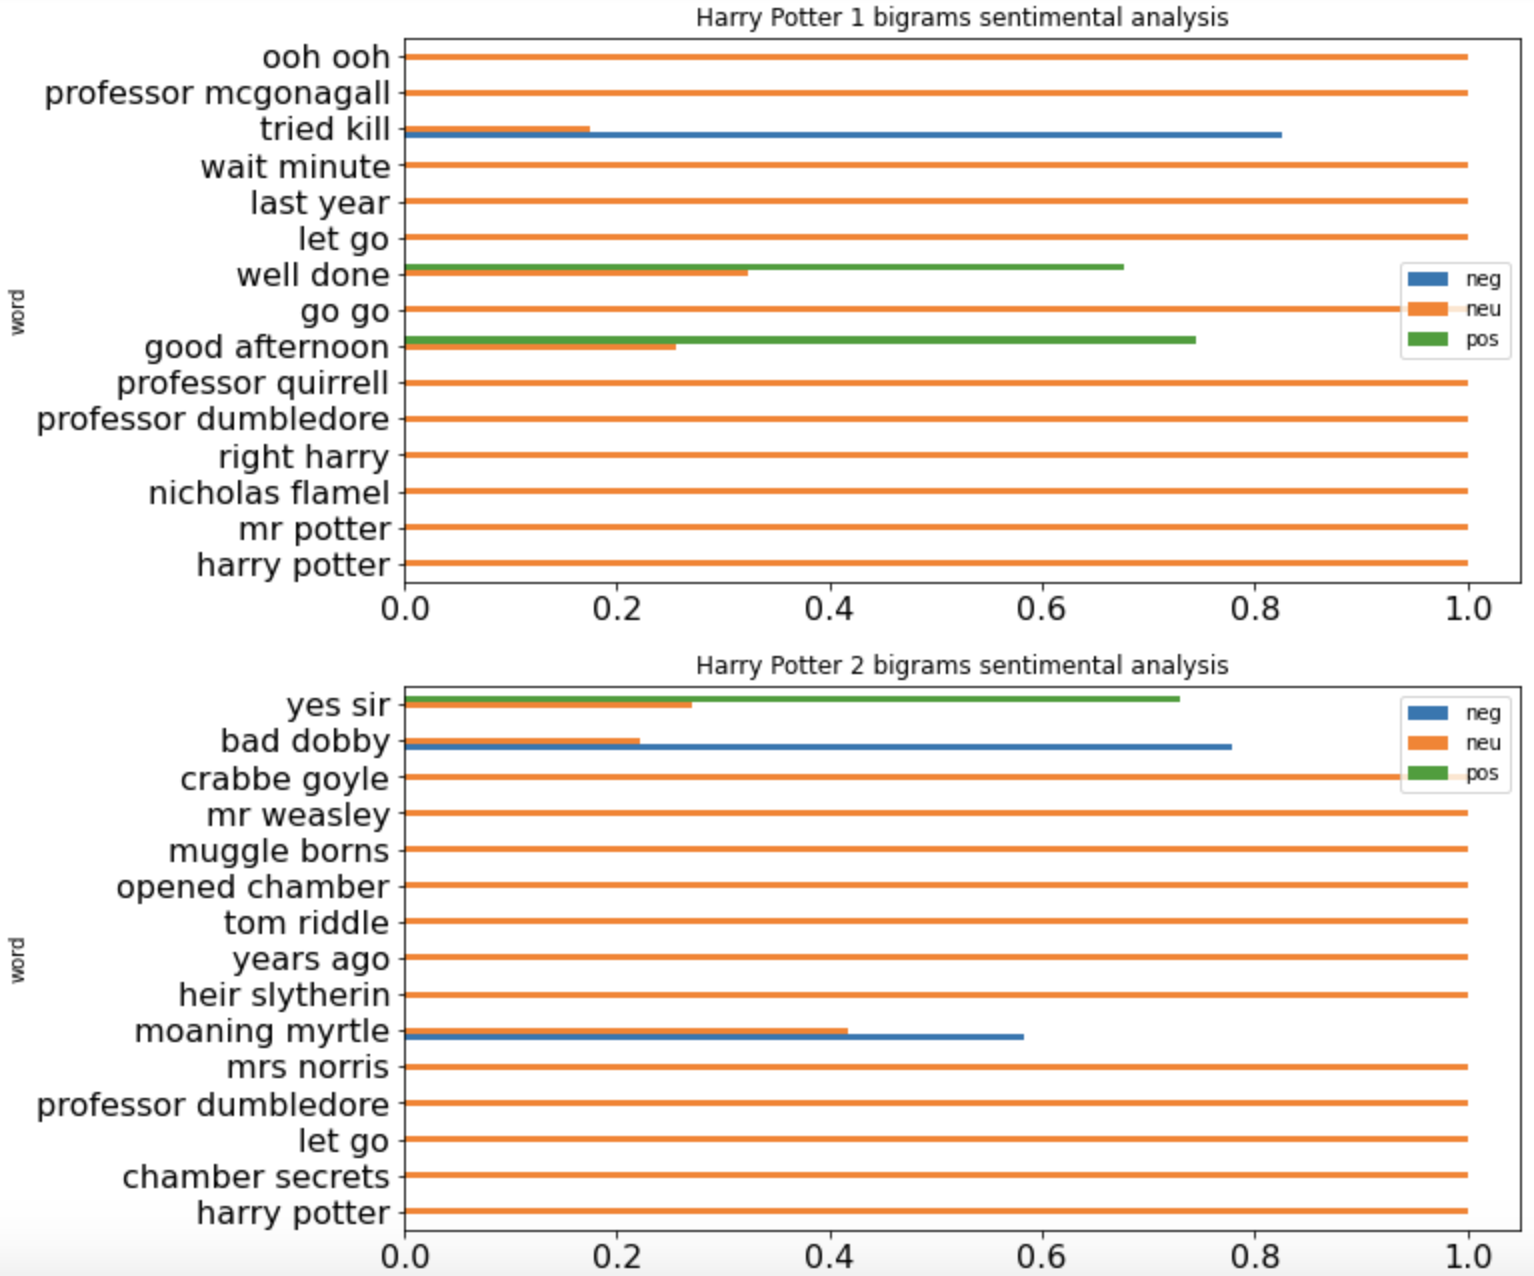
\includegraphics[width= 15 cm]{./figures/Bigrams_emotions.png}
    \caption{Analyse des émotions par bigrammes}
    \label{bigramemo}
\end{figure}
\FloatBarrier
\begin{figure}[hbt!]
    \centering
    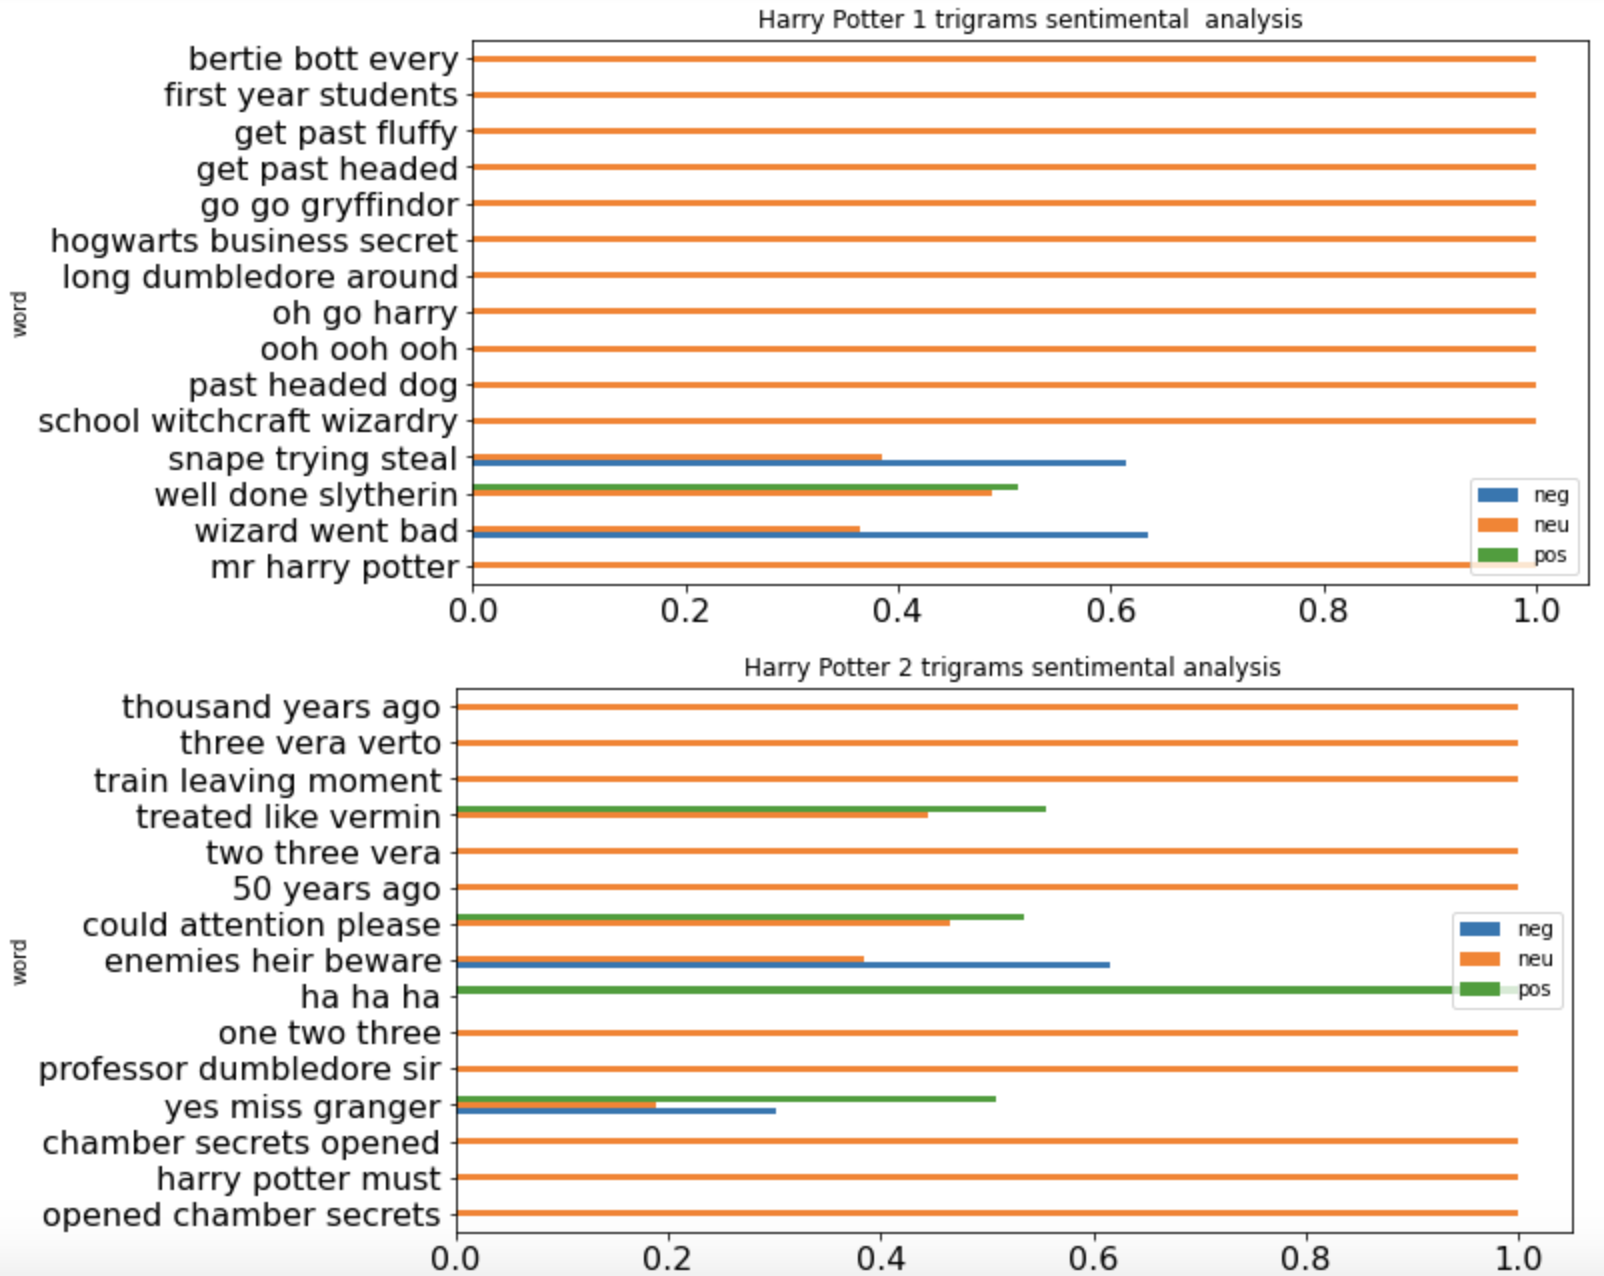
\includegraphics[width= 15 cm]{./figures/Trigrams_emotions.png}
    \caption{Analyse des émotions par trigrammes}
    \label{trigramemo}
\end{figure}
\FloatBarrier

Les Figures \ref{bigramemo} et \ref{trigramemo} montrent que la majorité des n-grammes extraits ont une polarité neutre, ce qui ne rajoute pas d'information sur le comportement individuel des personnages et général des maisons. Pour cela, nous allons plus loin dans cette analyse en extrayant des sentiments plus profonds tels que la colère, la peur, etc.\par

NRCLeX est une bibliothèque Python qui contient un dictionnaire des affects avec environ vingt-sept mille mots et qui se base sur le lexique des affects du Conseil National de Recherches du Canada (CNRC) et sur les ensembles des synonymes Wordnet de la bibliothèque \textit{NLTK}.
Dans le cadre de cette analyse préliminaire, nous utilisons cette bibliothèque pour générer les émotions à partir d'un corps de texte vue la difficulté de construire un modèle dédié à cette analyse.
Les affects émotionnels mesurés par NRCLeX sont : la peur, la colère, l'anticipation, la confiance, la surprise, la positivité, la négativité, la tristesse, le dégoût et la joie.\par

La figure \ref{emotions} représente les différentes émotions pour chaque maison, mesurées à partir du discours des personnages qui y appartiennent.

\begin{figure}[hbt!]
    \centering
    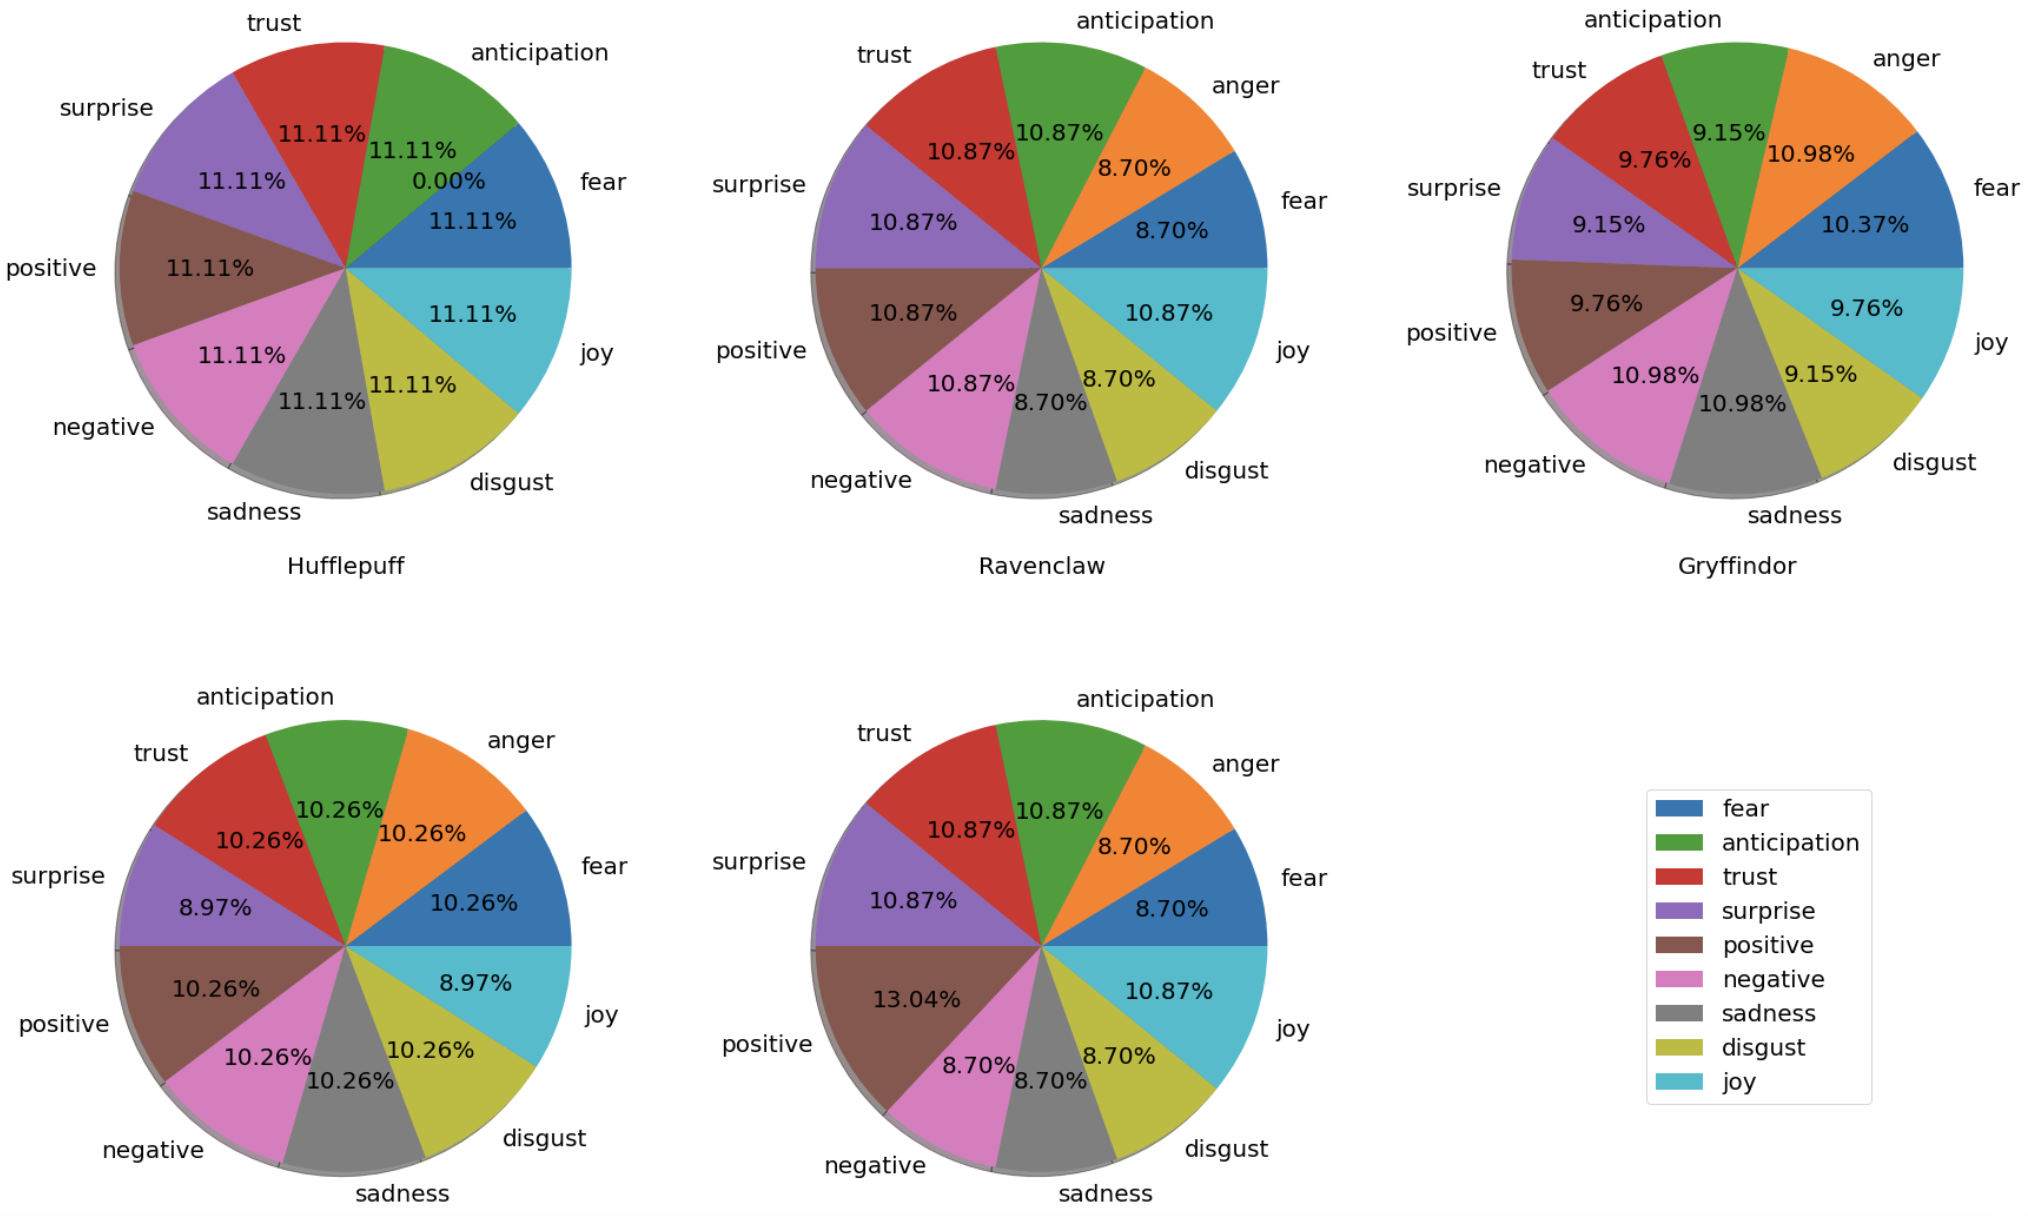
\includegraphics[width= 17 cm]{./figures/emotions_houses.png}
    \caption{Analyse des émotions par maison}
    \label{emotions}
\end{figure}
\FloatBarrier

Nous remarquons que la colère est une émotion non-exprimée par les personnages de la maison "Hufflepuff".
De plus, le comportement émotionnel général de la maison "Slytherin" s'oppose à celui de "Gryffindor" ; principalement au niveau des émotions "positive", "négative", "sadness" et "anger". D'autre part, ce comportement est quasiment similaire à celui de la maison "Ravenclaw" sauf au niveau de la positivité et la négativité.\par

\newpage

\subsubsection{Evaluation du modèle :}

Nous proposons une nouvelle matrice de design qui se constitue des connaissances sentimentales précédemment décrites, en plus du genre et du statut sanguin. Cette matrice est utilisée entièrement pour entraîner un modèle k-NN avec un nombre de voisins égal à 3.
Par la suite, nous avons utilisé la matrice du troisième film pour tester notre modèle.
\begin{figure}[hbt!]
    \centering
    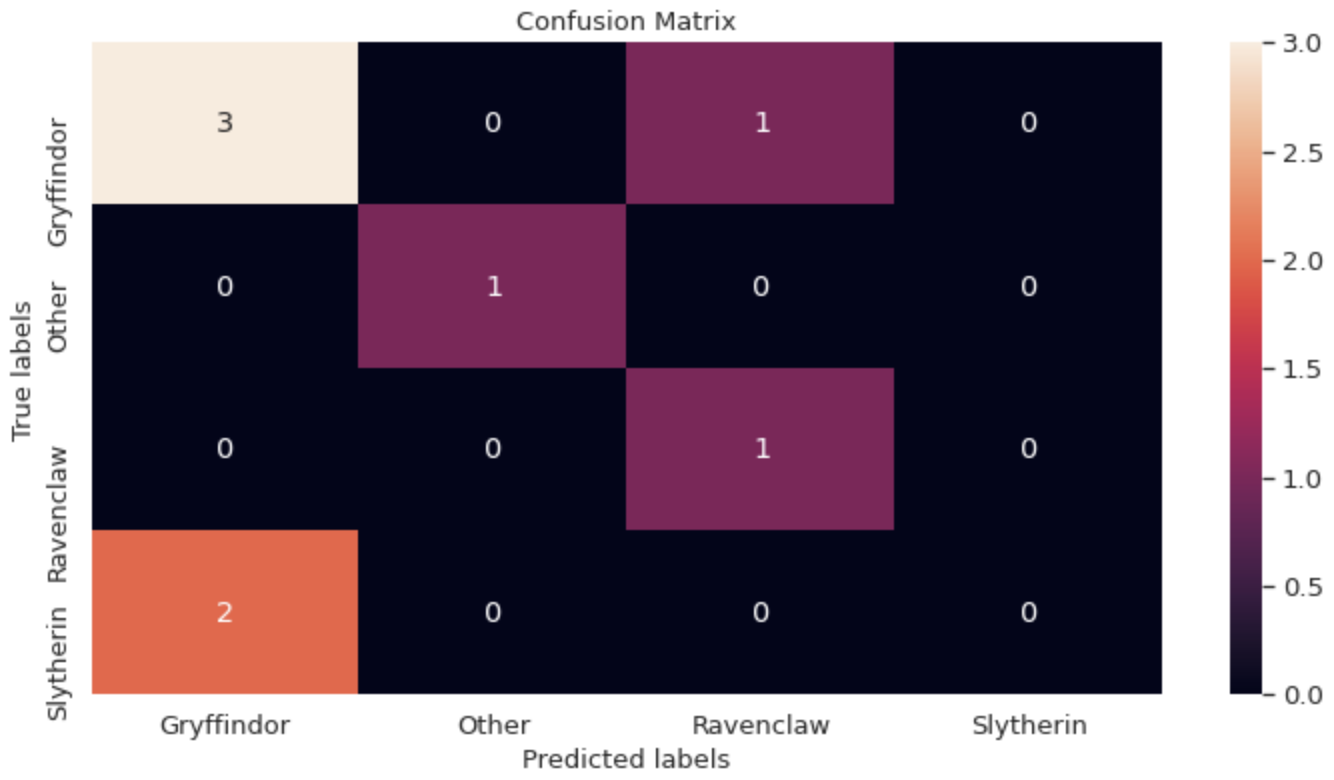
\includegraphics[width = 14 cm]{figures/matriceconfEmotions.png}
    \caption{Matrice de confusion}
    \label{matriceconfemo}
\end{figure}
\FloatBarrier

Nous remarquons que la précision du modèle a pu atteindre plus de 61\% sur les données du troisième film, contrairement aux modèles entraînés dans la section \ref{AN} où elle n'a pas depassé 50\%. Ces résultats encourageants ouvrent une perspective à explorer dans les prochain travaux sur ces données. Cependant, une limitation envisagée durant l’implémentation de cette approche consiste à l'élimination de plusieurs personnages ; soit qui n'expriment pas des émotions ou qui n'ont pas de discours. Cette limitation minimise le nombre de données d'entraînement, ce qui nous a obligé à utiliser toutes les données extraites des films 1 et 2 pour l'entraînement et celles du troisième film pour le test.\par

\newpage

%-----------------------------------------------------------%
\subsection{Annexe 2 : Dépôt Git du projet}\label{A2}
%-----------------------------------------------------------%

L'ensemble du code est présent sur le dépôt Git du projet à l'adresse suivante : \\ \url{https://github.com/BascouFlorent/Classification_Personnage_2021.git}

\newpage

\printbibliography[
heading=bibintoc,
] %Prints the entire bibliography with the title "Whole bibliography"

\end{document}
